\chapter{高层视觉处理:从视觉到认知} \label{chap:chap24}

如我们所见,低级视觉处理负责在投影到视网膜上的光模式下检测各种形式的对比度。
中级处理与鉴定所谓的视觉原语,例如运动和运动场以及表面隔离。
高级视觉处理整合了来自各种来源的信息,是导致视觉感知的视觉途径的最后阶段。


高级视觉处理与识别环境的行为有意义的特征有关,因此取决于从短期工作记忆,长期记忆和大脑皮层执行区域传达信息的下降信号。


\section{高级视觉处理与对象识别有关}

我们对世界的视觉体验从根本上以对象为中心。
即使在视网膜上施放在视网膜上的光线图案时,我们也可以识别相同的对象,而随着照明,角度,位置和距离等观看条件的差异很大。
即使对于视觉上复杂的对象,也是如此,这些对象包括大量连接的视觉特征。


此外,物体不仅仅是视觉实体,而是与特定的体验,其他记忆的物体和感觉(例如咖啡研磨机的嗡嗡声或情人香水的香气)以及各种情感相关的。
对象的行为意义是基于视觉信息引导我们的行动的。
简而言之,对象识别在视力和认知之间建立了联系(图 ~\ref{fig:24_1})。


\begin{figure}[htbp]
	\centering
	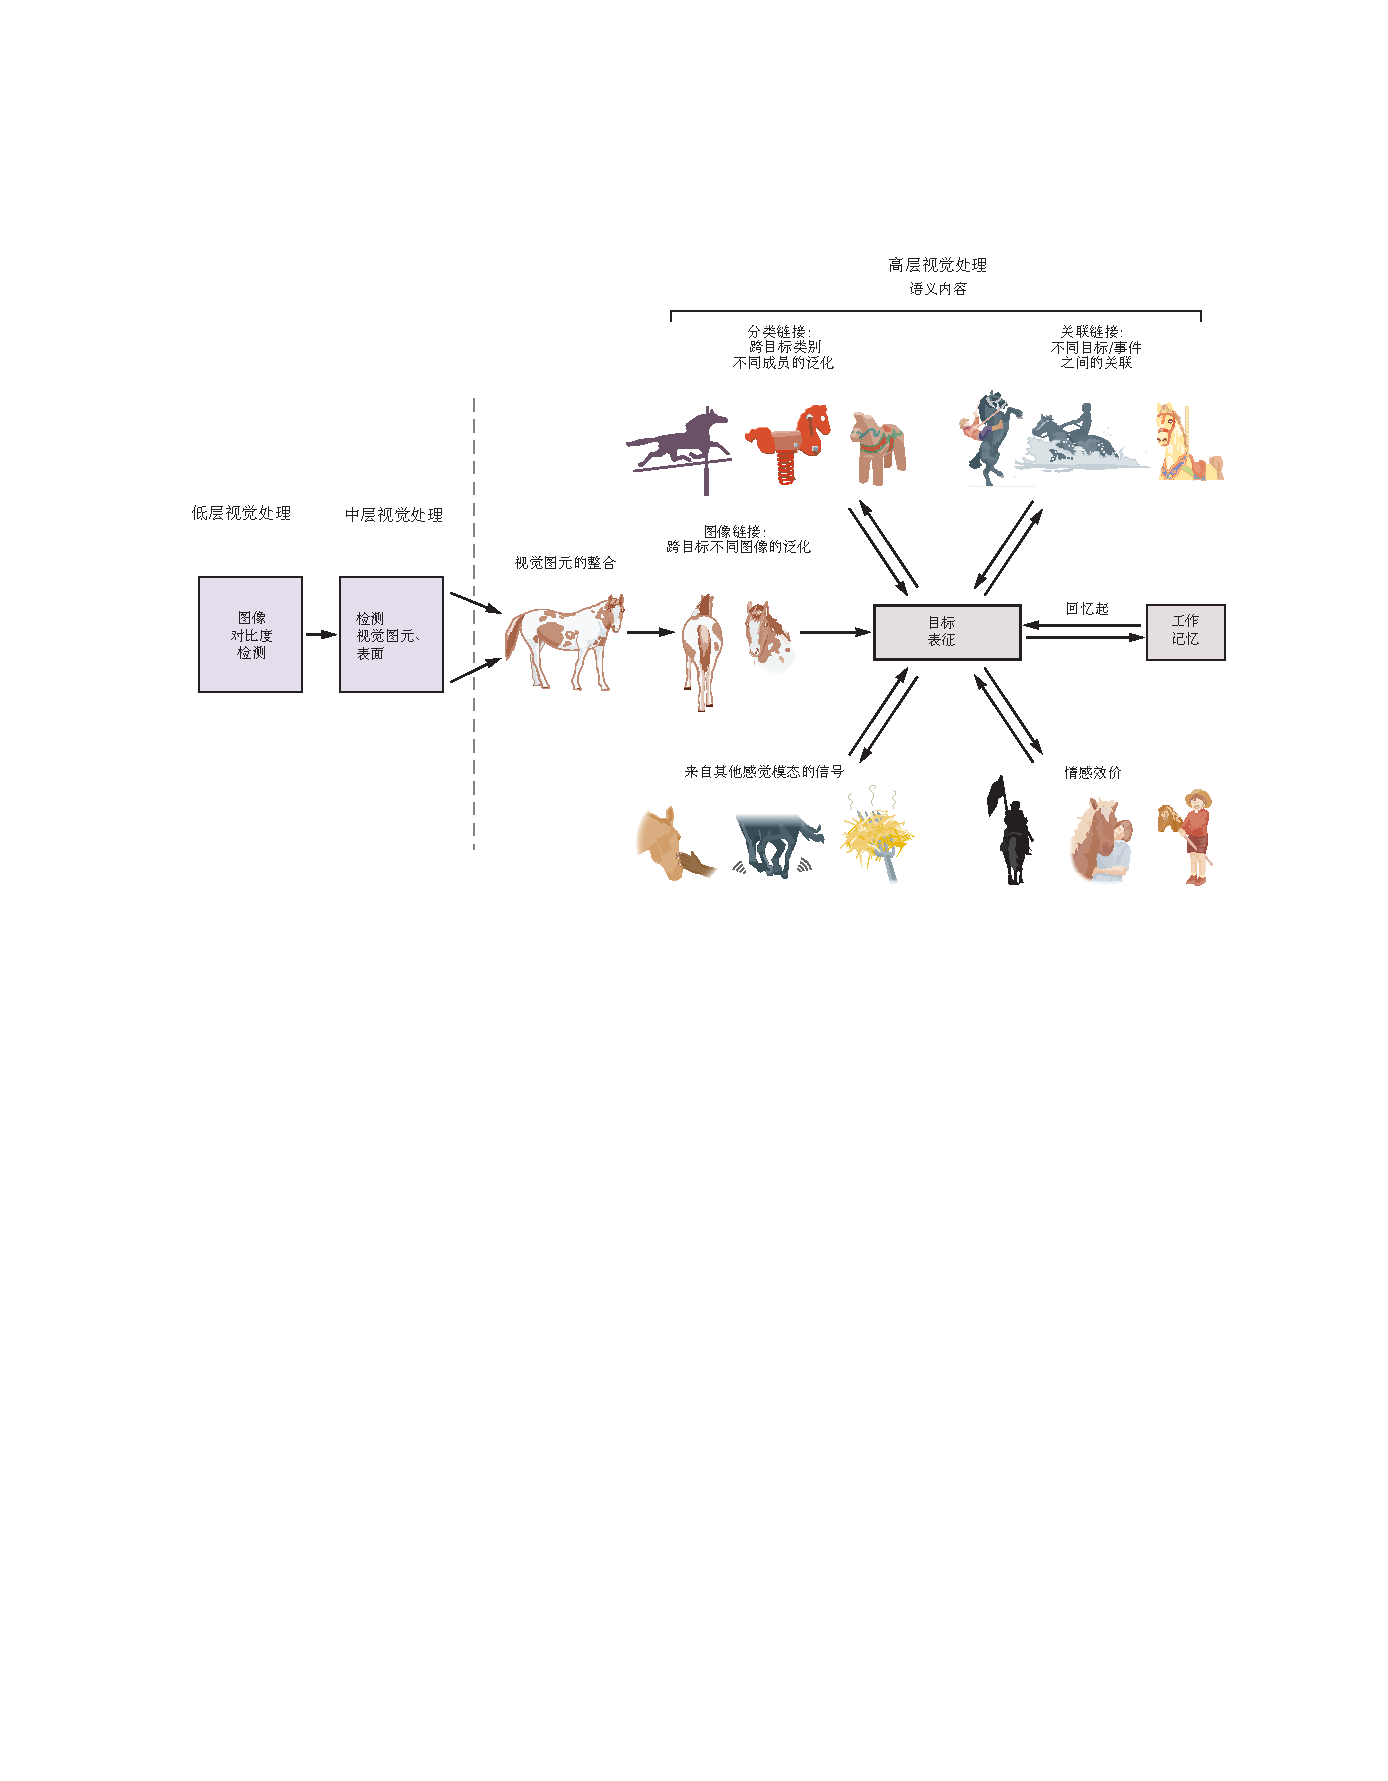
\includegraphics[width=0.9\linewidth]{chap24/fig_24_1}
	\caption{整个对象的表示是高级视觉处理的核心。 整个对象的表示涉及在视觉通路的早期阶段提取的视觉特征的整合。 这种整合是由同一对象和对象类别的不同成员生成的大量视网膜图像的概括。 该表示还结合了来自其他感官模式的信息,附加情感效价,并将该对象与其他对象或事件的记忆相关联。 对象表示可以存储在工作记忆中,并与其他记忆相关联地回忆起来。}
	\label{fig:24_1}
\end{figure}



\section{下颞叶皮层是物体识别的主要中心}

灵长类动物研究暗示颞叶的新皮层区域,主要是颞叶皮层,在物体感知中。
由于皮层视觉系统中突触中继的层次结构从主要的视觉皮层延伸到颞叶,因此颞叶是许多类型的视觉信息收敛的位置。


神经心理学研究发现,对颞颞皮层的损害会产生特定的物体识别失败。
神经生理和功能成像研究反过来又对下颞神经元的活性代表对象,这些表示与感知和认知事件的关系以及如何通过经验进行修饰的方式产生了显着的见解。


源自视网膜中的视觉信号在达到初级视觉皮层之前,在丘脑的侧向核核中进行处理。
初级视觉皮层的上行视觉途径遵循两个主要的平行和分层组织的流:腹侧和背面流(第~\ref{chap:chap21}~ 章)。
腹侧流从初级视觉皮层到V2向腹侧延伸到下颞皮层,在猕猴中,该皮层包括上颞沟的下库和颞叶的腹侧凸度(图24-2)。
该腹流中每个突触继电器的神经元从前阶段接收收敛输入。
在层次结构的顶部,下颞神经元可以在广泛的视觉空间区域整合大量的视觉信息。


\begin{figure}[htbp]
	\centering
	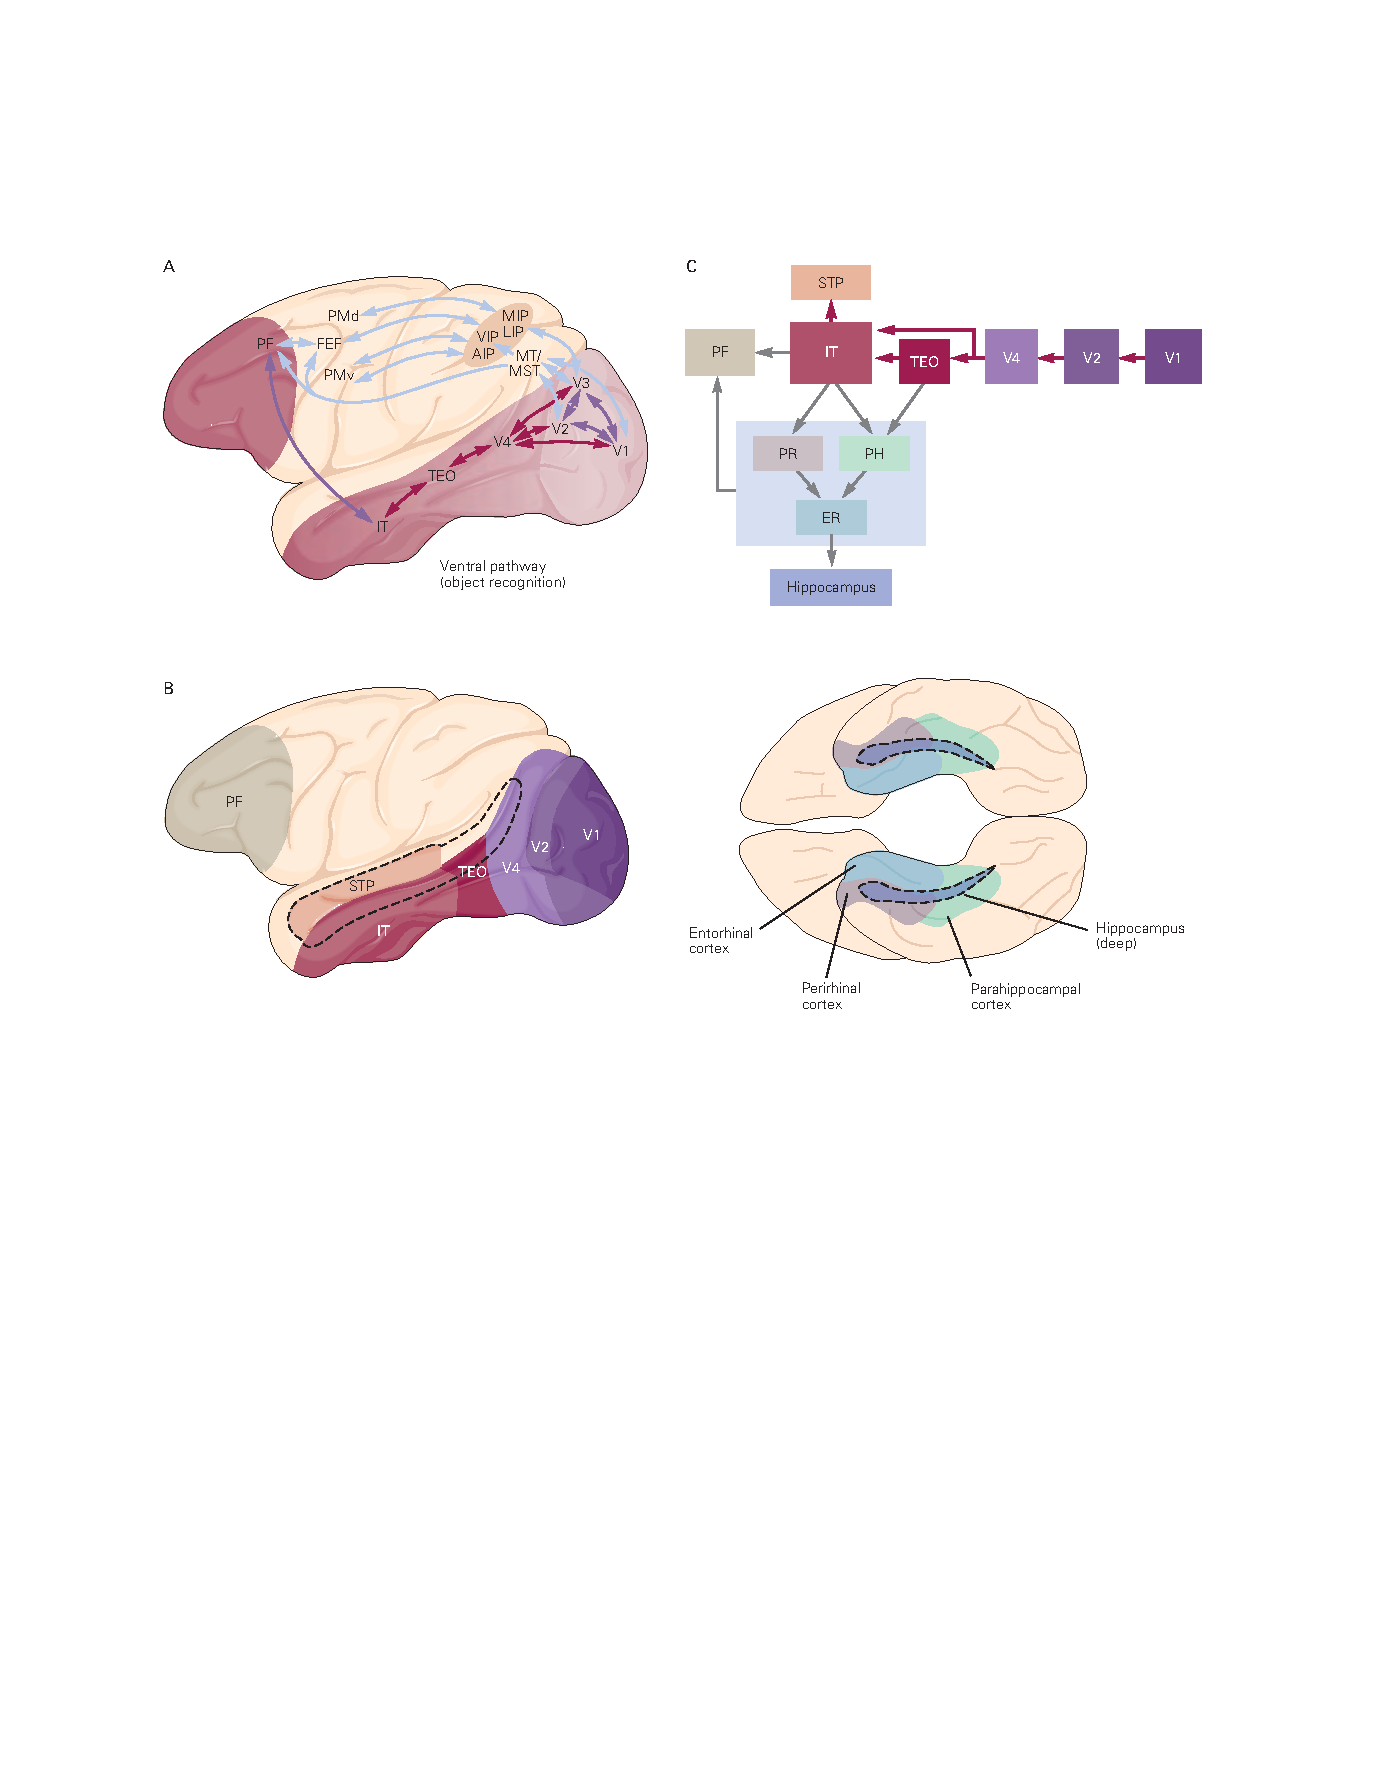
\includegraphics[width=0.95\linewidth]{chap24/fig_24_2}
	\caption{物体识别的皮层通路。
		A. 猕猴大脑的侧视图显示了涉及视觉处理的主要通路,包括物体识别通路(红色)。
		(缩写:AIP,前顶内皮层;FEF,额叶视野;IT,颞下皮层;LIP,外侧顶内皮层;MIP,内侧顶内皮层;MST,内侧颞上皮层;MT,中颞叶皮层;PF,前额叶皮层 ;PMd,背侧前运动皮层;PMv,腹侧前运动皮层;TEO,颞枕叶皮层;VIP,腹侧顶内皮层。)
		B. 猕猴大脑的侧视图和腹侧视图显示参与物体识别的皮层区域。
		(缩写:IT,颞下皮层;PF,前额叶皮层;STP,颞上多感觉区;TEO,颞枕叶皮层。)
		C. 颞下皮层 (IT) 是腹侧流的末期(红色箭头) 并与内侧颞叶和前额叶皮层(灰色箭头)的相邻区域相互连接。 
		此图表说明了信息流的主要连接和主要方向。 
		(缩写:ER,内嗅皮质;PF,前额皮质;PH,海马旁皮层;PR,鼻周皮层;STP,颞上多感觉区;TEO,颞枕皮层。)}
	\label{fig:24_2}
\end{figure}


下颞皮层是大脑区域。
与该区域的解剖连接的模式表明,它至少包括两个主要的功能细分 - 后枕骨后皮质和前区域颞皮层 - 功能证据表明,进一步分别属于多个功能专长的区域。
正如我们将看到的那样,神经心理学和神经生理学证据支持下颞皮层的前部和后部部分之间的区别。



\subsection{临床证据表明颞下皮层对于物体识别至关重要}

在19世纪后期,当美国神经学家桑格·布朗(Sanger Brown)和英国生理学家爱德华·阿尔伯特·施弗(EdwardAlbertSchäfer)发现,灵长类动物的实验性病变废除了识别对象的能力,对介导对象识别的神经途径的第一个明确见解是获得了。
与枕叶区域病变伴随的缺陷不同,颞叶病变不会损害对基本视觉属性(例如颜色,运动和距离)的敏感性。
由于视觉丧失的类型,这种损害最初被称为心理失明,但此术语后来被视觉上的agnosia(“无视觉知识”)取代,这是由Sigmund Freud创造的术语。


在人类中,有两个基本类别的视觉不适,具有敏感性和联想性,其描述导致了视觉系统中对象识别的两个阶段模型。
有了具有敏感性的不可思议,匹配或复制复杂的视觉形状或对象的能力受到损害(图~\ref{fig:24_3})。
这种障碍是由于对象识别的第一阶段的破坏而引起的:将视觉特征集成到整个对象的感觉表示中。
借助关联的不可思议,匹配或复制复杂对象的能力仍然完好无损,但是识别对象的能力受到损害。
这种障碍是由于对象识别的第二阶段的破坏而引起的:对象的感官表示与对象的含义或功能的了解的关联。


\begin{figure}[htbp]
	\centering
	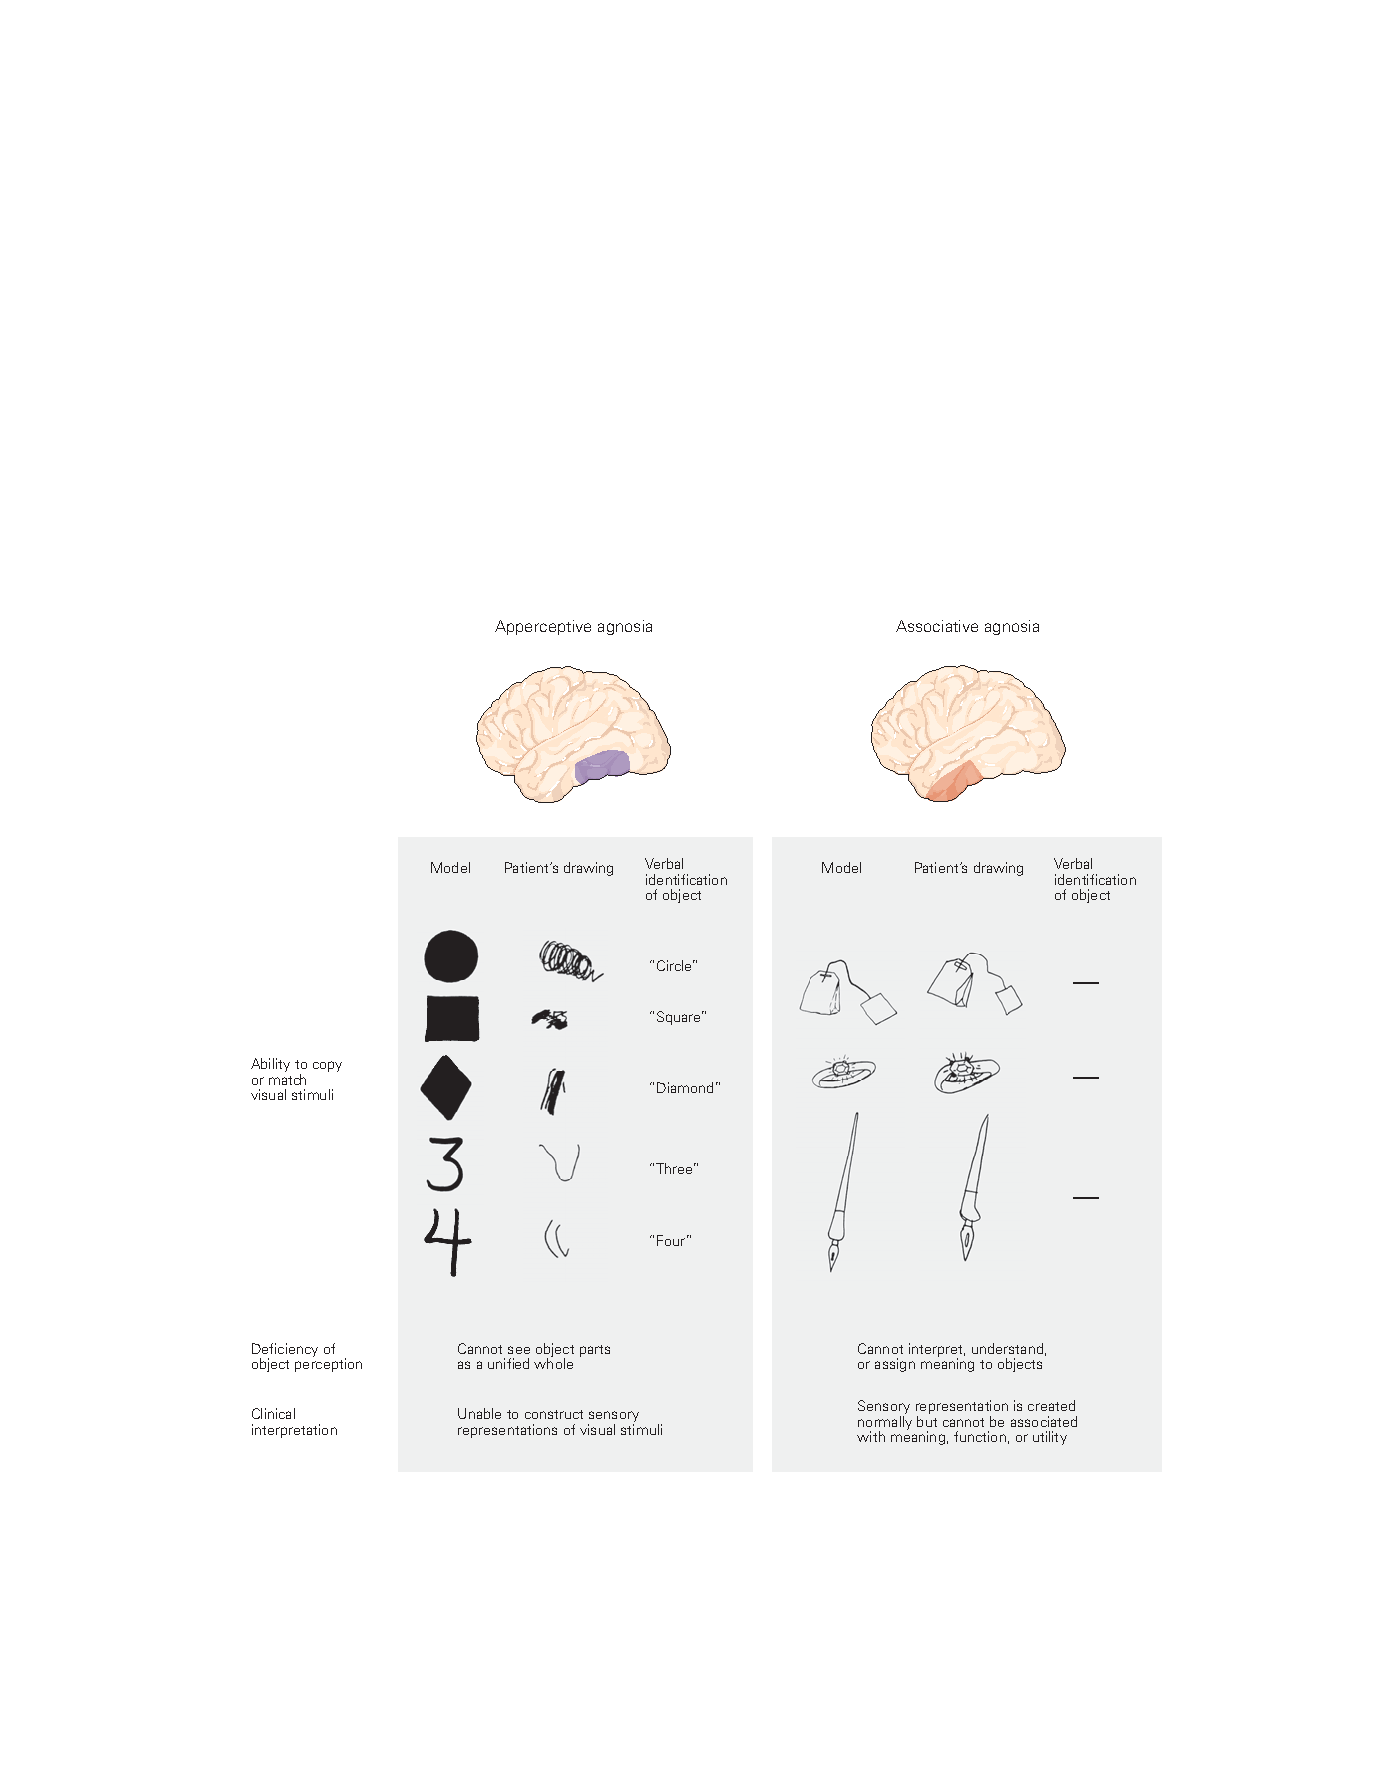
\includegraphics[width=0.8\linewidth]{chap24/fig_24_3}
	\caption{人类颞叶中的神经元参与物体识别。下颞叶皮层受损会削弱识别视觉对象的能力,这种情况称为视觉失认症。 有两大类视觉失认症:后部区域受损导致的知觉性失认症和前部区域受损导致的联想性失认症。 (经许可转载自 Farah 1990。© 1990 麻省理工学院。)}
	\label{fig:24_3}
\end{figure}


与该功能性层次结构一致,在颞下颞皮层损害后,具有敏感性的女性是最常见的,而在颞下颞皮层损害的损害之后,缔合性不足是一种高阶感知缺陷。
前细分中的神经元表现出在后部区域未见的各种与记忆相关的特性。


颞皮层中更多的焦点病变会导致特定的缺陷。
对人类颞叶的一小部分区域的损害导致无法识别面部,这是一种称为prosopagnosia的联想性毒死的形式。
Prosopagnosia患者可以将面部识别为脸部,识别其部分,甚至检测到面部表达的特定情绪,但他们无法将特定的面孔识别为属于特定人的脸。


Prosopagnosia是类别特定类别的不可思议的一个例子,其中颞叶损伤的患者无法识别属于特定语义类别的特定项目。
还报道了针对生物,水果,蔬菜,工具或动物的特定类别的不症。
由于面部的明显行为意义以及人们认识到大量面孔的正常能力,Prosopagnosia可能只是最常见的特定类别特异性的agnosia。



\subsection{下颞叶皮层中的神经元编码复杂的视觉刺激,并按功能专门的列组织}

从1970年代查尔斯·格罗斯(Charles Gross)和同事的工作开始,已经对颞叶中的视觉信息进行编码进行了广泛的研究。
该区域的神经元具有独特的响应特性。
它们对简单的刺激特征(例如方向和颜色)相对不敏感。 
取而代之的是,绝大多数人具有较大的中心位置接收场,并编码复杂的刺激特征。
这些选择性通常看起来有些任意。
例如,单个神经元可能会对特定颜色和质地的新月形模式做出强烈反应。
具有独特选择性的细胞可能会为对特定有意义对象的响应的高阶神经元提供输入。


实际上,在下颞皮层中,正面有意义的物体(例如面部和手)激活了几个小的神经元亚群(图~\ref{fig:24_4}),如查尔斯·格罗斯(Charles Gross)所发现的那样。
对于响应手视线的细胞,单个手指特别关键。
在响应面部的细胞中,某些细胞的最有效刺激是面部的正面视图,而对于其他细胞来说,这是侧视图。
尽管某些神经元一般对面孔的反应优先,但另一些神经元仅对特定的面部表情做出反应。
这种细胞似乎直接有助于面对识别。


\begin{figure}[htbp]
	\centering
	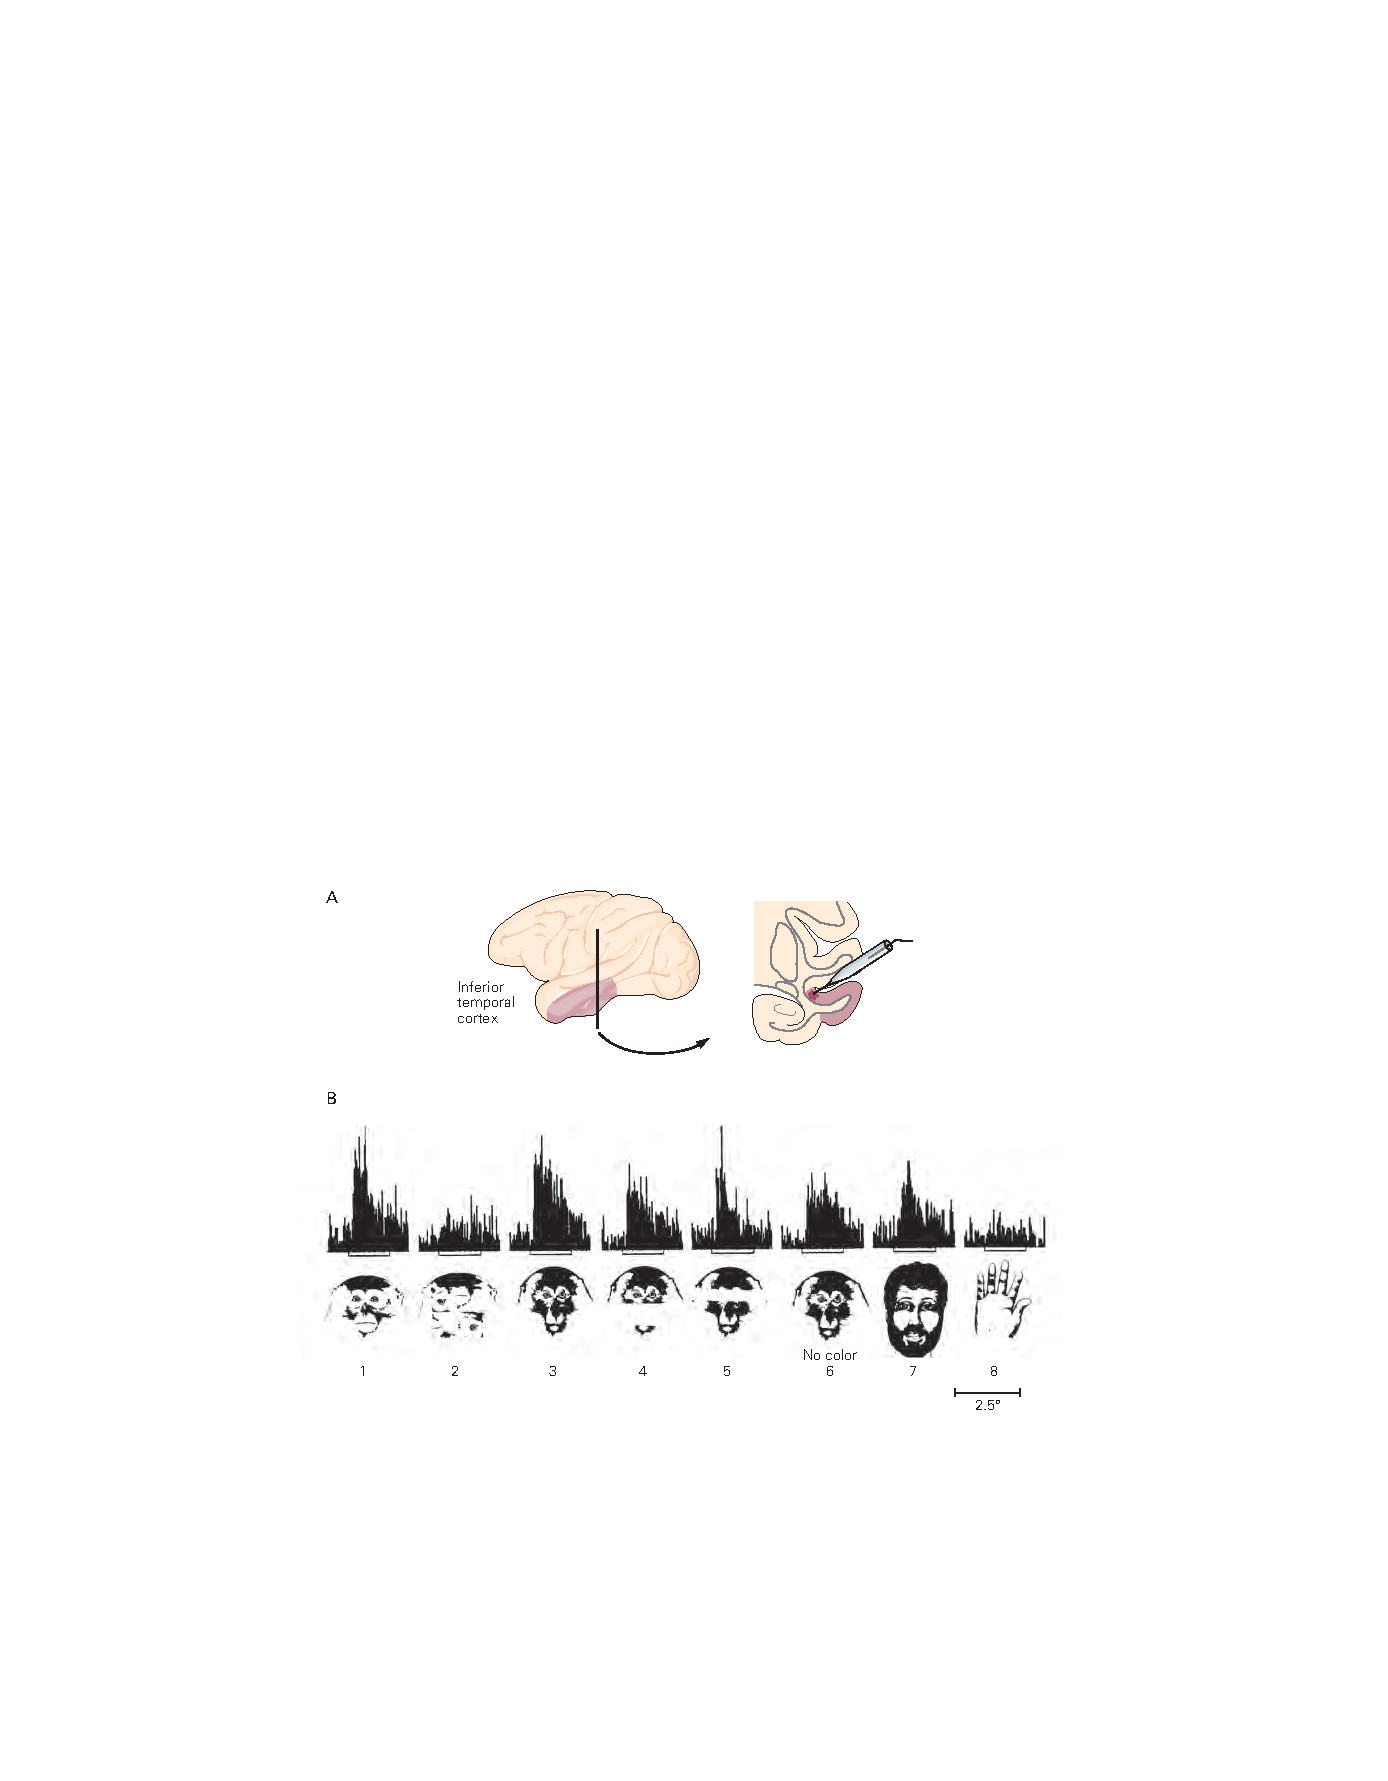
\includegraphics[width=0.7\linewidth]{chap24/fig_24_4}
	\caption{猴子颞下皮层的神经元参与面部识别。 (经许可转载自 Desimone 等人,1984 年。版权所有 © 1984 年神经科学协会。) 
		A. 猴子颞下皮层的位置显示在侧视图和冠状剖面中。 彩色区域是记录神经元的位置。 
		B. Peristimulus 时间直方图说明了单个神经元中动作电位的频率以响应不同的图像(显示在直方图下方)。
		这个神经元选择性地对面孔做出反应。
		遮盖关键特征,例如嘴巴或眼睛 (4, 5),会导致反应显着但并非完全减少。
		扰乱面部 (2) 的各个部分几乎消除了反应。}
	\label{fig:24_4}
\end{figure}


在皮层视觉系统的初始继电器中,对相同的刺激特征响应的神经元,例如方向或运动方向,但在视野的不同部分中响起。
下颞皮层内的细胞类似地组织了。
代表相同或相似刺激特性的神经元的列通常延伸到整个皮层厚度,并在约400μm的范围内延伸。
排列的列是使具有某些相似特征的不同刺激在部分重叠的列中表示的(图~\ref{fig:24_5})。
因此,一个刺激可以激活多个列。
水平连接可以跨越许多毫米,并可能促进用于编码对象的分布式网络的形成。


\begin{figure}[htbp]
	\centering
	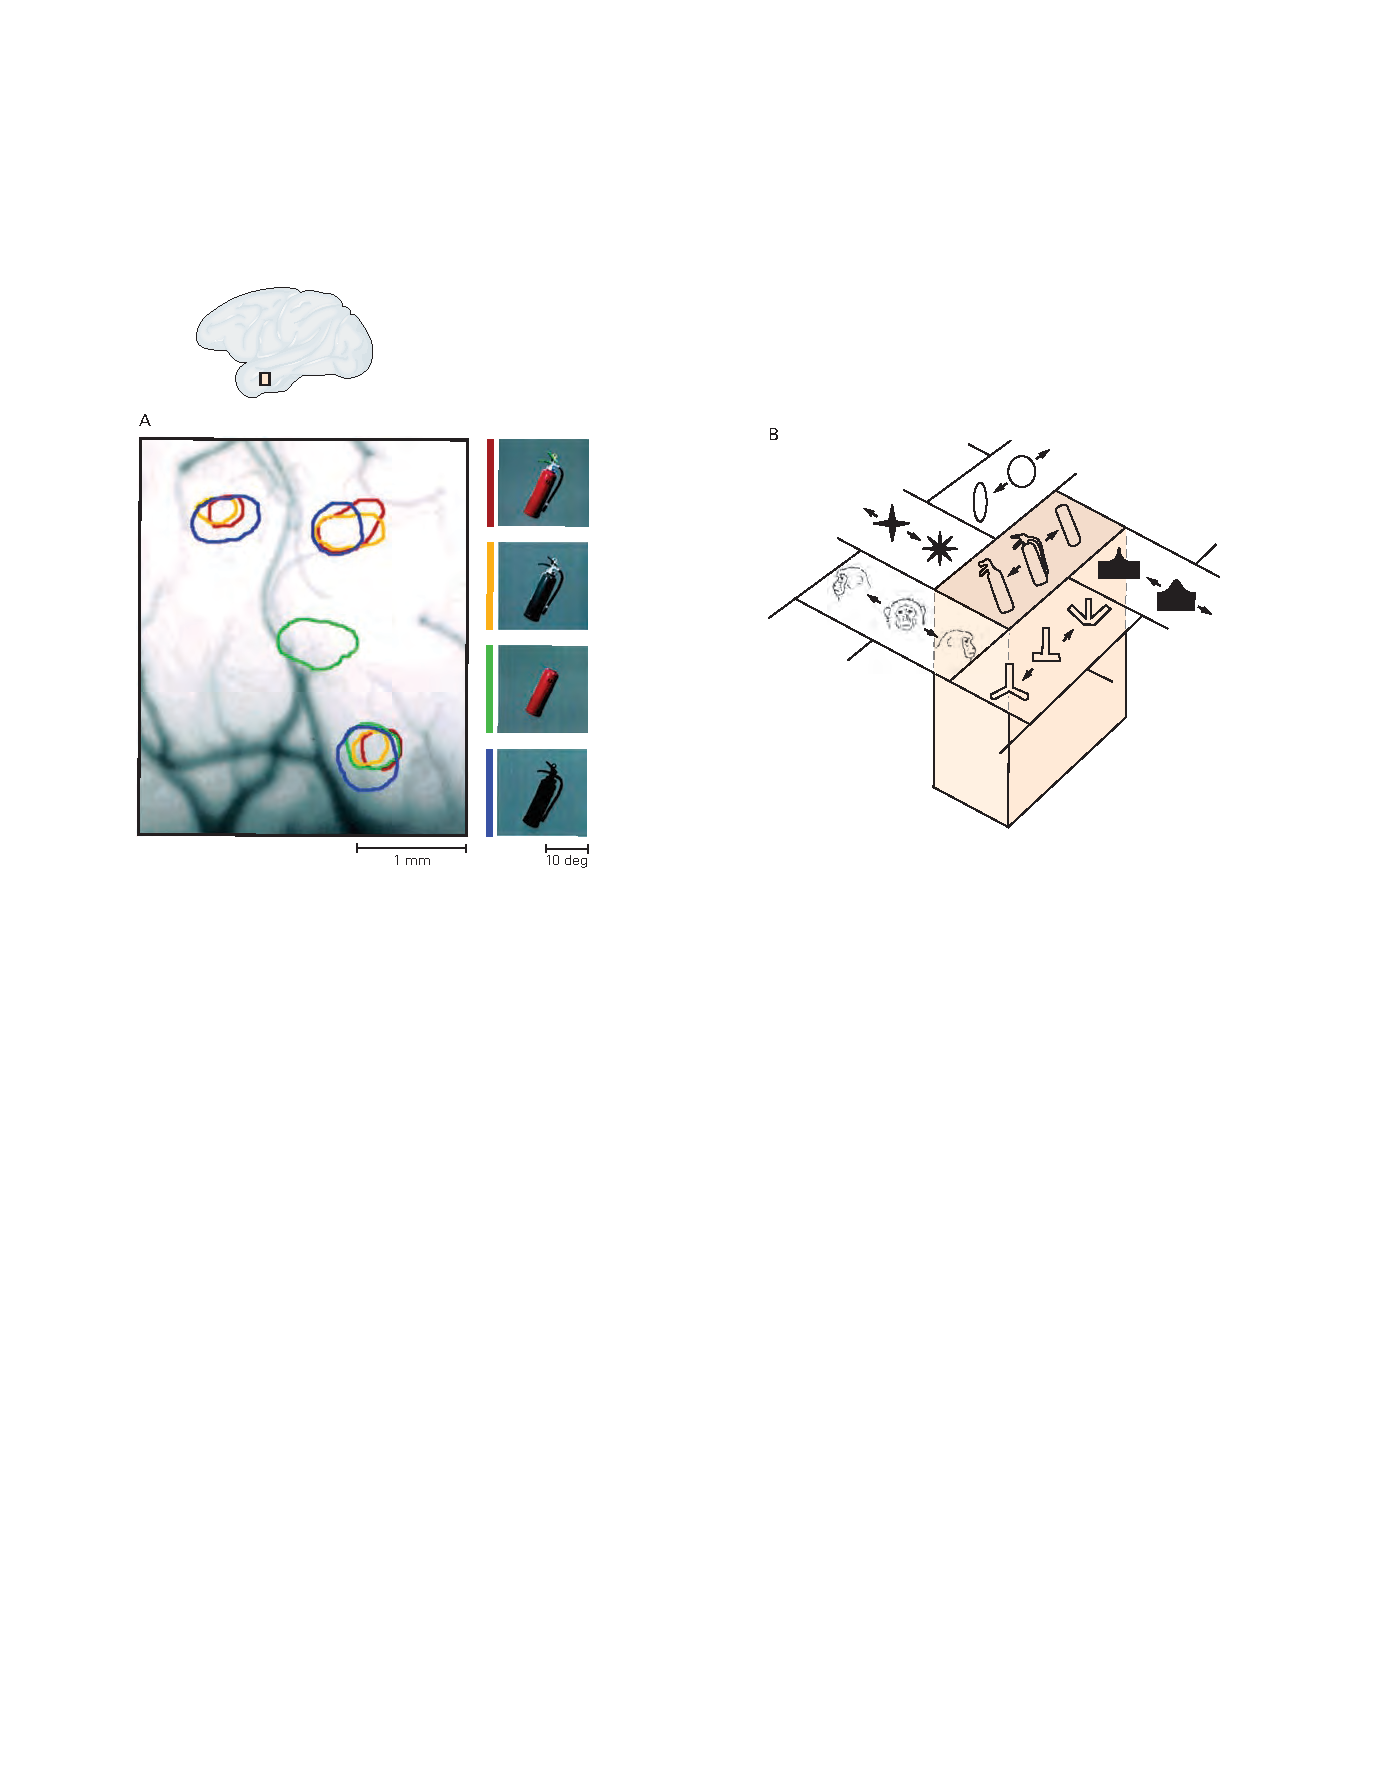
\includegraphics[width=0.5\linewidth]{chap24/fig_24_5}
	\caption{下颞叶皮层前部对复杂视觉刺激作出反应的神经元被组织成列。 (经许可转载自 Tanaka 2003。版权所有 © 2003 Oxford University Press。) A. 前下颞叶皮层表面的光学图像说明了被右侧所示物体选择性激活的区域。 B. 下颞叶皮层的神经元组织成从皮层表面延伸出来的功能特化的列。 根据这个模型,每一列都包含对特定视觉复杂对象做出反应的神经元。 代表一个对象的变化的神经元列,例如不同的面孔或不同的灭火器,构成了一个超列。}
	\label{fig:24_5}
\end{figure}



\subsection{灵长类动物的大脑包含用于面部处理的专用系统}

普通话通常发生在没有任何其他形式的不可思议的情况下。
如此高度特异性的感知赤字可以通过位于独家簇中的面部选择性神经元的局灶性病变来解释。
Nancy Kanwisher和同事使用\textit{功能性磁共振成像}以及Gregory McCarthy和Gregory McCarthy和同事使用来自人脑表面的直接电生理记录来加强这种想法。
Kanwisher及其同事发现,与其他物体相比,在面部叶状面部面积的一个区域和其他物体的图像和其他物体的图片和其他物体的一个区域相比,在面部呈现过程中的反应要大得多。


随后,发现了更多的面部选择区域,主要是在时间上,但也位于前额叶皮层中。
对这些领域的早期研究为面部选择性神经元聚集提供了间接证据。
在后来的研究中,多丽丝·托索(Doris Tsao),温里希·弗莱瓦尔德(Winrich Freiwald)和同事直接证明了这种聚类,并表明面部处理可能是由从下颞皮层后部到前额叶皮层的专用面部处理网络进行的。
他们使用\textit{功能性磁共振成像},在颞皮层中发现了六个区域,在猕猴的前额叶皮层中发现了三个区域,对面部的反应比对其他物体更有选择性。
这些区域(称为面部斑块)在个人的位置高度一致的位置发现,因此根据其位置命名。
每个脸部斑块的直径为几毫米,因此与下时间柱有组织不同。
脸部斑块的细胞内记录表明,绝大多数细胞对面的反应比对其他物体的反应更多。
因此,将数百万的面细胞聚集成固定数量的小区域。
这些区域是直接连接的,从而形成了面部处理网络。
在此网络中,每个节点似乎都在功能上专业化。
从颞叶内的后部到前部位置,初始脸部贴片对面部的特定视图做出反应,然后面部斑块逐渐对身份更具选择性,而对视角的选择性更少。 
此外,颞叶内的背侧面积对自然面部运动具有选择性,而腹侧面积缺乏。
因此,一个高度专业的网络主要位于颞皮层,处理面部传达的信息的多个维度(图~\ref{fig:24_6})。


\begin{figure}[htbp]
	\centering
	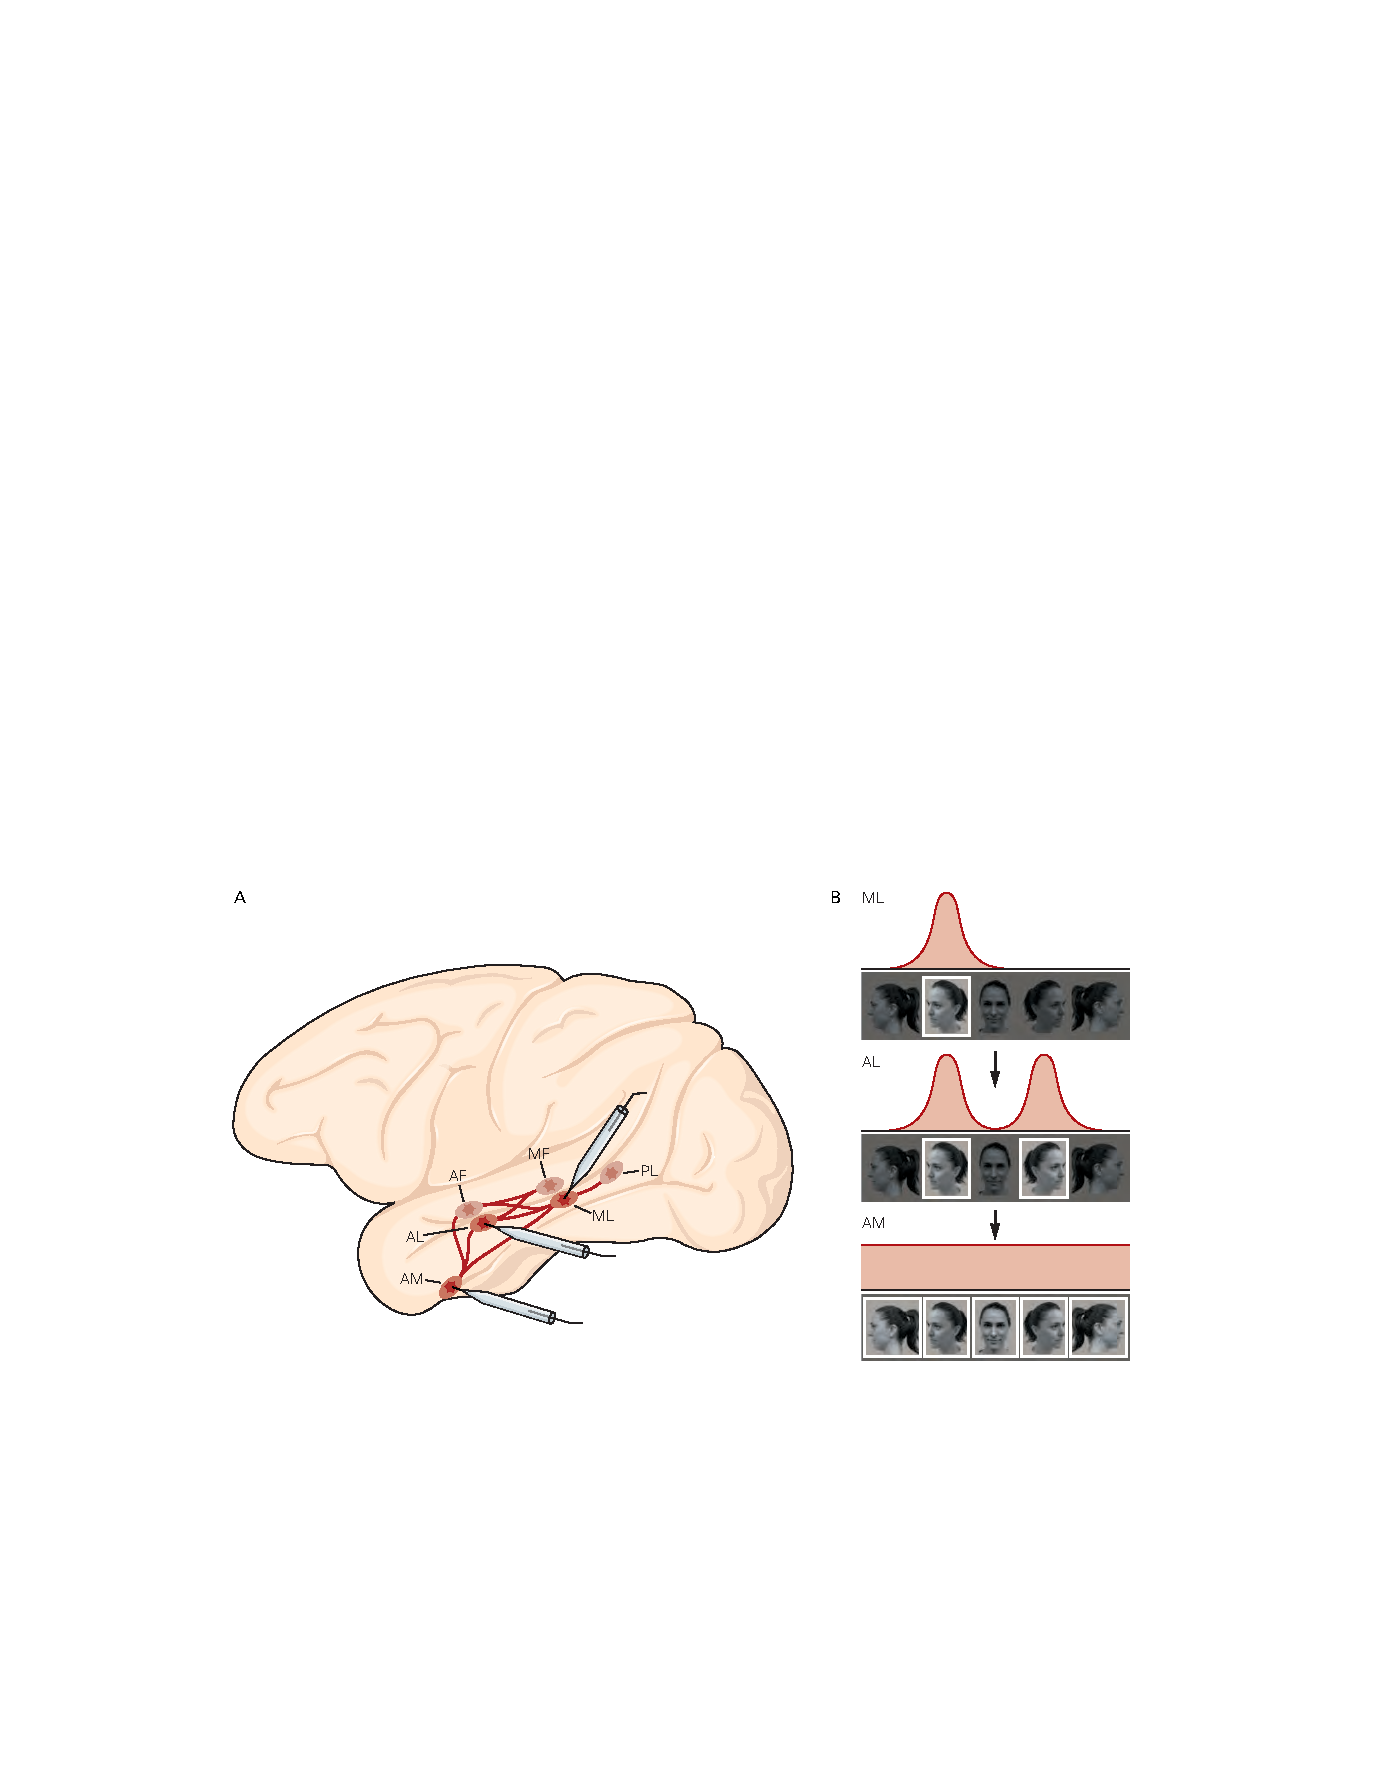
\includegraphics[width=0.9\linewidth]{chap24/fig_24_6}
	\caption{颞叶包含面部选择性区域网络。A. 猕猴观看面部和其他物体图片的功能磁共振成像识别了颞叶、颞上沟内部和周围的六个面部选择性区域。这些区域出现在不同受试者的相同位置,并根据其解剖位置命名(PL,后外侧;ML,内侧外侧;MF,颞上沟内侧底;AL,前外侧;AF,前眼底; AM,前内侧)。这些区域相互连接形成一个人脸处理网络。B. 来自 ML、AL 和 AM 区域的单神经元记录显示调整到头部方向。 ML 细胞被调整到特定的头部方向,许多 AL 细胞被调整到彼此镜像对称版本的多个方向,而 AM 细胞被广泛地和更弱地调整到头部方向。 互连区域中的这三种表示可以被认为是彼此的转换(箭头)。}
	\label{fig:24_6}
\end{figure}



\subsection{下颞叶皮层是参与物体识别的皮层区域网络的一部分}

对象识别与视觉分类,视觉记忆和情感密切相互交织,而下颞皮层的输出会导致这些功能(见图24-2)。
主要投影中有向临时皮质的周围和偏头皮皮层的投影,它们位于颞下皮层的腹侧表面(图24-2C)。
这些区域反过来又投影到内嗅皮层和海马形成,这两者都参与了长期记忆存储和检索。
下颞皮层的第二个主要投影是前额叶皮层,这是高级视觉处理的重要部位。
正如我们将看到的那样,前额叶神经元在对象分类,视觉工作记忆和内存回忆中起重要作用。


下颞皮层还向杏仁核直接和间接地通过直接和间接地通过杏仁核提供了输入,据信,杏仁核可以将情感价应用于感觉刺激并参与情感的认知和内脏成分(第~\ref{chap:chap42}~章)。
最后,下颞皮层是皮质多模式感觉区域的主要输入来源,例如上颞型多突增工区(图~\ref{fig:24_2}B),该区域位于与下颞皮层相邻的背面。



\section{物体识别依赖于感知恒常性}

尽管有时有明显不同的视网膜图像,但在不同的观看条件下将对象识别为相同的能力是视觉体验功能上最重要的要求之一。
对象的不变属性(例如,图像特征或特征特征(例如斑马的条纹)之间的空间和色素关系)是对象的身份和含义的提示。


为了进行对象识别,这些不变属性必须独立于其他图像属性表示。
视觉系统可以熟练地做到这一点,其行为表现称为感知恒定。
感知恒定的形式从跨对象的简单转换(例如大小或位置的变化)到更困难的形式,例如深度旋转或照明的变化,甚至是类别中对象的相同性:所有: 斑马看起来像一样。


最好的例子之一是尺寸恒定。
与观察者不同距离处的对象被认为具有相同的大小,即使对象在视网膜上产生不同绝对大小的图像。
数百年来,大小的构成已被认可,但仅在过去几十年中,才有可能确定负责的神经机制。
一项早期的研究发现,颞皮层下的病变会导致猴子大小恒定的失败,这表明该区域的神经元在大小恒定体中起着至关重要的作用。
确实,个体下颞神经元最引人注目的特性之一是它们的形状选择性甚至对刺激大小的很大变化的变化(图~\ref{fig:24_7}A)。


感知恒定的另一种类型是位置稳定性,其中对象被识别为相同的位置,而不管它们在视野中的位置如何。
当对象在其大型接收场中改变位置时,许多下颞神经元的选择性反应模式不会有所不同(图~\ref{fig:24_7}b)。
形式 - 提示不变性是指定义形式变化的提示时形式的恒定。
例如,亚伯拉罕·林肯(Abraham Lincoln)头部的轮廓都可以识别出是黑色,白色的黑色,还是绿色的红色。 
许多下颞神经元的反应不会随着对比度的变化(图~\ref{fig:24_7}C),颜色或纹理而变化。


\begin{figure}[htbp]
	\centering
	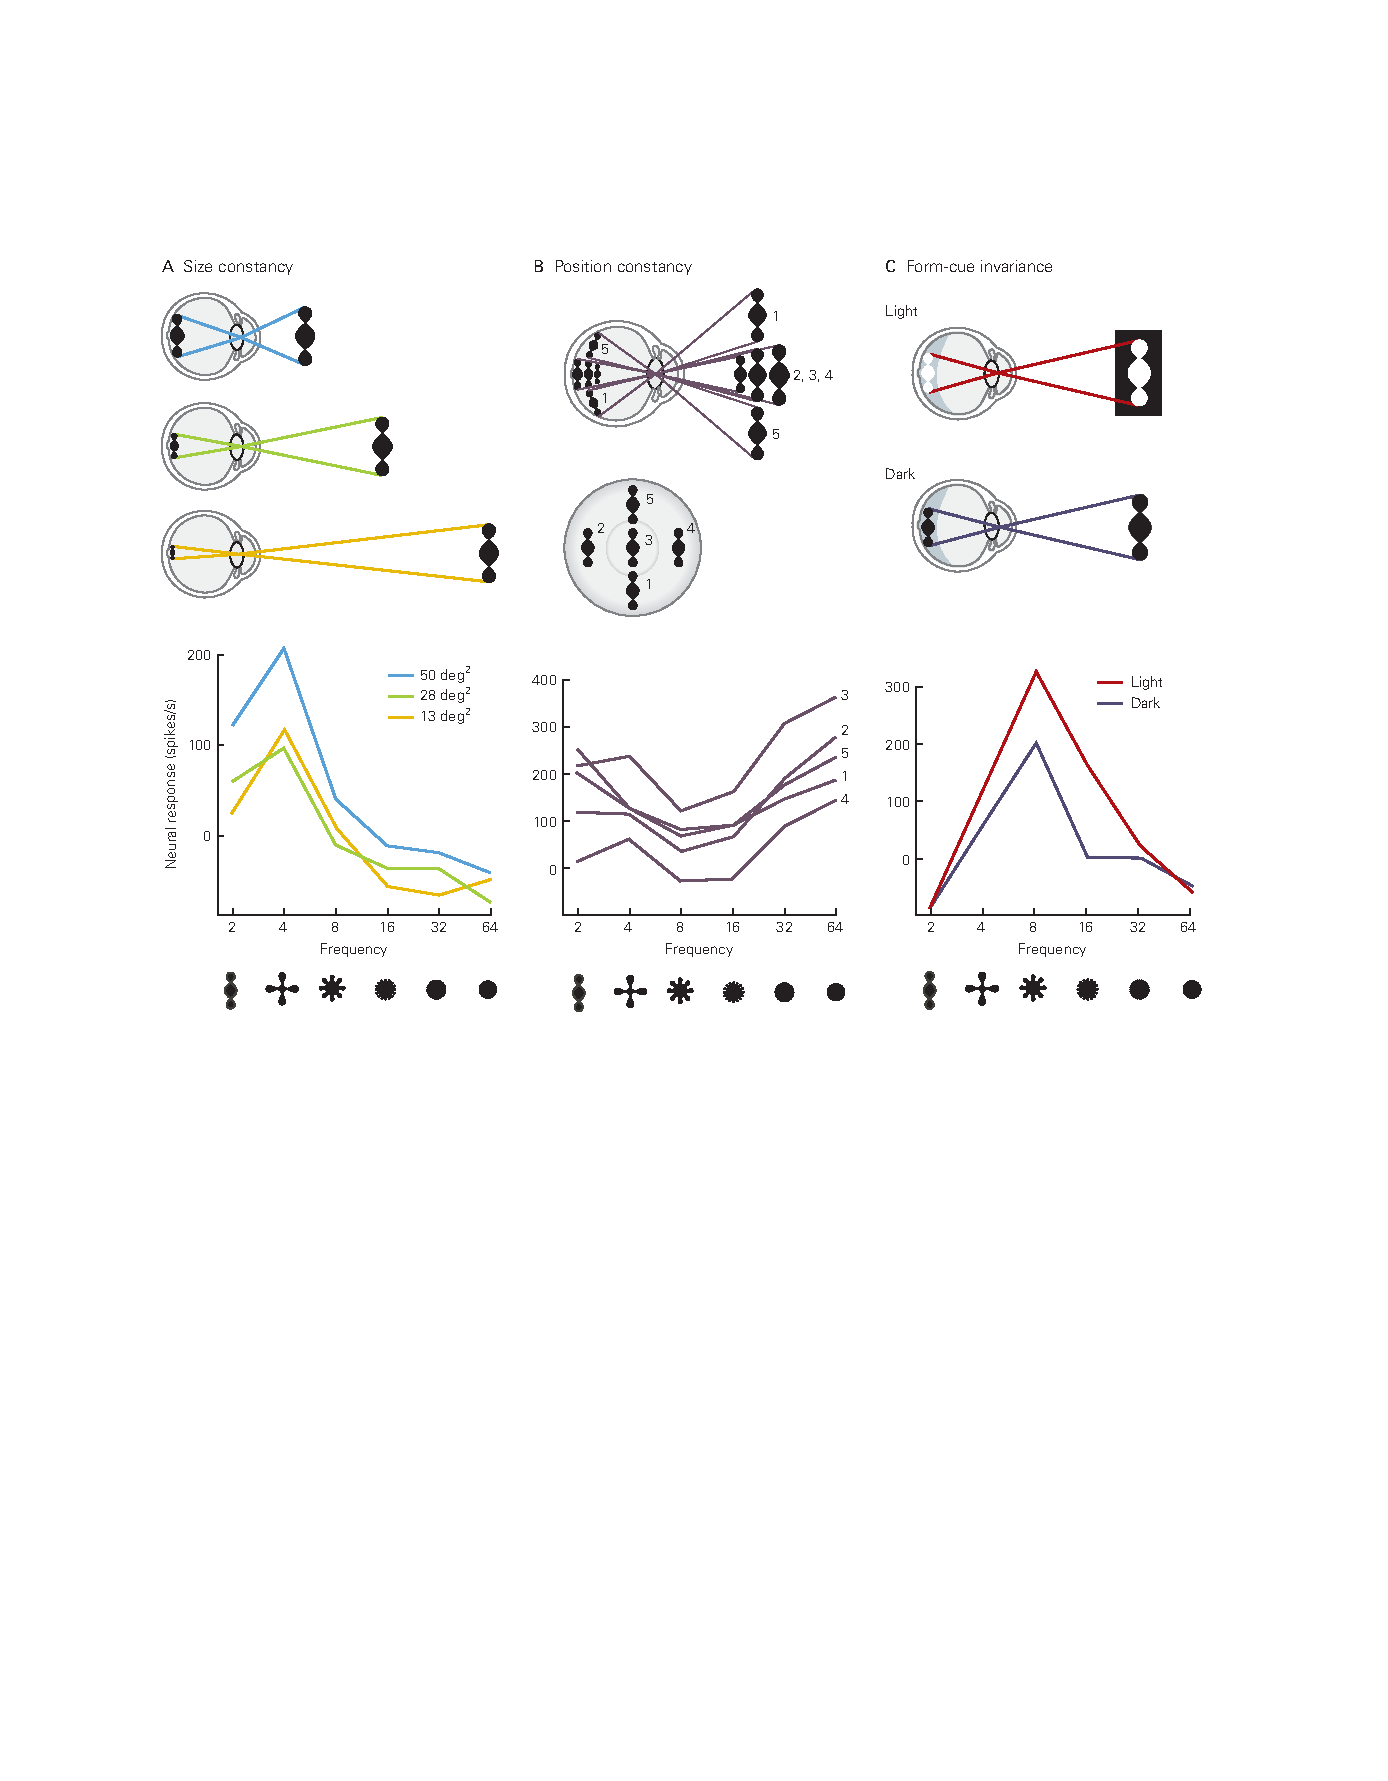
\includegraphics[width=0.9\linewidth]{chap24/fig_24_7}
	\caption{知觉恒常性反映在颞下皮层神经元的行为中。 许多下颞叶神经元的反应对具有特定频率(数量)的叶的刺激具有选择性,但不随物体大小、位置和反射率变化。 (经许可转载自 Schwartz 等人,1983 年。) A. 尺寸恒定性。 即使视网膜图像的大小随着视野中物体的距离而减小,物体也会被感知为相同的。 绝大多数下颞叶神经元对视网膜图像大小显着变化的反应是不变的,如此处单个细胞的记录所示。 B. 位置不变。 尽管视网膜图像中的位置发生变化,但物体仍被认为是相同的。 几乎所有下颞叶神经元对视野中不同位置的相同刺激都有类似的反应,如此处单个神经元的记录所示。 C. 形式提示不变性。 尽管反射率发生变化,但物体仍被认为是相同的。 如单个神经元的记录所示,大多数下颞叶神经元对所示的两个图像的反应相似。}
	\label{fig:24_7}
\end{figure}


视角不变性是指从不同角度观察到的三维对象的感知恒定。
因为我们看到的大多数物体都是三维和不透明的,当从不同的角度看时,有些部分变得不可见,而其他部分则被揭示,而其他所有部分都会在外观变化。
然而,尽管可能由熟悉的物体施放的无限视网膜图像范围,但观察者可以轻松地独立于观察其角度识别对象。
该规则有明显的例外,通常是在从一个产生非特征性的视网膜图像的角度查看对象的情况下发生的,例如从上方直接查看的桶。


因此,对象识别机制必须从明显的复杂形状中推断对象的身份。
下颞皮层中的许多神经元都不表现出视点不变性。
实际上,许多人系统地调整了视角。
然而,在较大的前部位置,神经元不仅大小和位置不变,而且对观点也表现出更大的不变性。
面部处理系统是一个很好的例子。
后面部斑块中的神经元被调整为视角,而前脸斑块中的神经元表现出极大的稳健性,可以改变视点的变化。
因此,与前部区域相比,后面面部区域中的人口反应包含有关头部方向的更多信息,而前脸斑块则提供了与后面部面积相比,有关跨头方向的更多信息。
神经元的个体神经元和种群在前下颞皮层中达到的观点不变性可能足以说明感知观点不变性。
但这尚未直接显示。
另外,可以在较高的皮层加工阶段(例如前额叶皮层)实现观点不变性。


研究观点不变性失败的条件可能会导致对行为神经机制的见解。
这样的条件是镜像图像的介绍。
尽管镜像不完全相同,但经常被认为是这样的混乱,反映了系统以识别视点不变性的错误阳性识别。
卡尔·奥尔森(Carl Olson)及其同事研究了下颞皮层特定区域中神经元对镜像图像的反应。
与感知混乱一致,许多下颞神经元对这两个图像的反应类似。
同样,在前面描述的后部和前部之间的一个面积中,剖面选择性细胞与面部的左和右谱相似。
这些结果加强了以下结论:下颞皮层中的活动反映了感知不变性,尽管在这种情况下是错误的,而不是刺激的实际特征。



\section{目标的分类感知简化了行为}

所有形式的感知恒定物都是视觉系统试图跨单个对象产生的不同视网膜图像的尝试的产物。
更一般的恒定类型是对单个对象的感知属于同一语义类别。
例如,篮子中的苹果或字母A的许多出现在不同字体上是物理上截然不同的,但毫不费力地认为是绝对相同的。


分类感知通常被定义为比同一类别的对象更好地区分不同类别的对象的能力。
例如,要区分两个红灯的波长占10纳米比区分相同波长差的红色和橙色灯要困难。


分类感知简化了行为。
例如,苹果是完全球形的还是左侧略微斑驳的,还是我们提供的座椅是温莎还是奇彭代尔的侧椅都无关紧要。
同样,阅读能力要求一个人能够识别多种类型样式的字母。
像更简单的感知恒定形式一样,分类感知取决于大脑提取所见对象不变特征的能力。


是否存在对类别中对象以及对不同类别对象的对象的均匀响应的神经元人群?
为了测试这一点,戴维·弗里德曼(David Freedman)和伯爵·米勒(Earl Miller)及其同事创建了一组图像,其中合并了狗和猫的特征。
复合图像中狗和猫的比例从一个极端到另一个极端变化。 
对猴子进行了训练,可以可靠地将这些刺激识别为狗或猫。
米勒及其同事随后从背外侧前额叶皮层中的视觉响应神经元记录,该区域从下颞皮层接收直接输入。
这些神经元不仅表现出预测的类别选择性反应 - 对猫的反应很好,但反之亦然,反之亦然,而且神经元类别边界也对应于行为学到的边界(图~\ref{fig:24_8})。 
相比之下,下颞皮层中的神经元代表特征的相似性,而不是类别。


\begin{figure}[htbp]
	\centering
	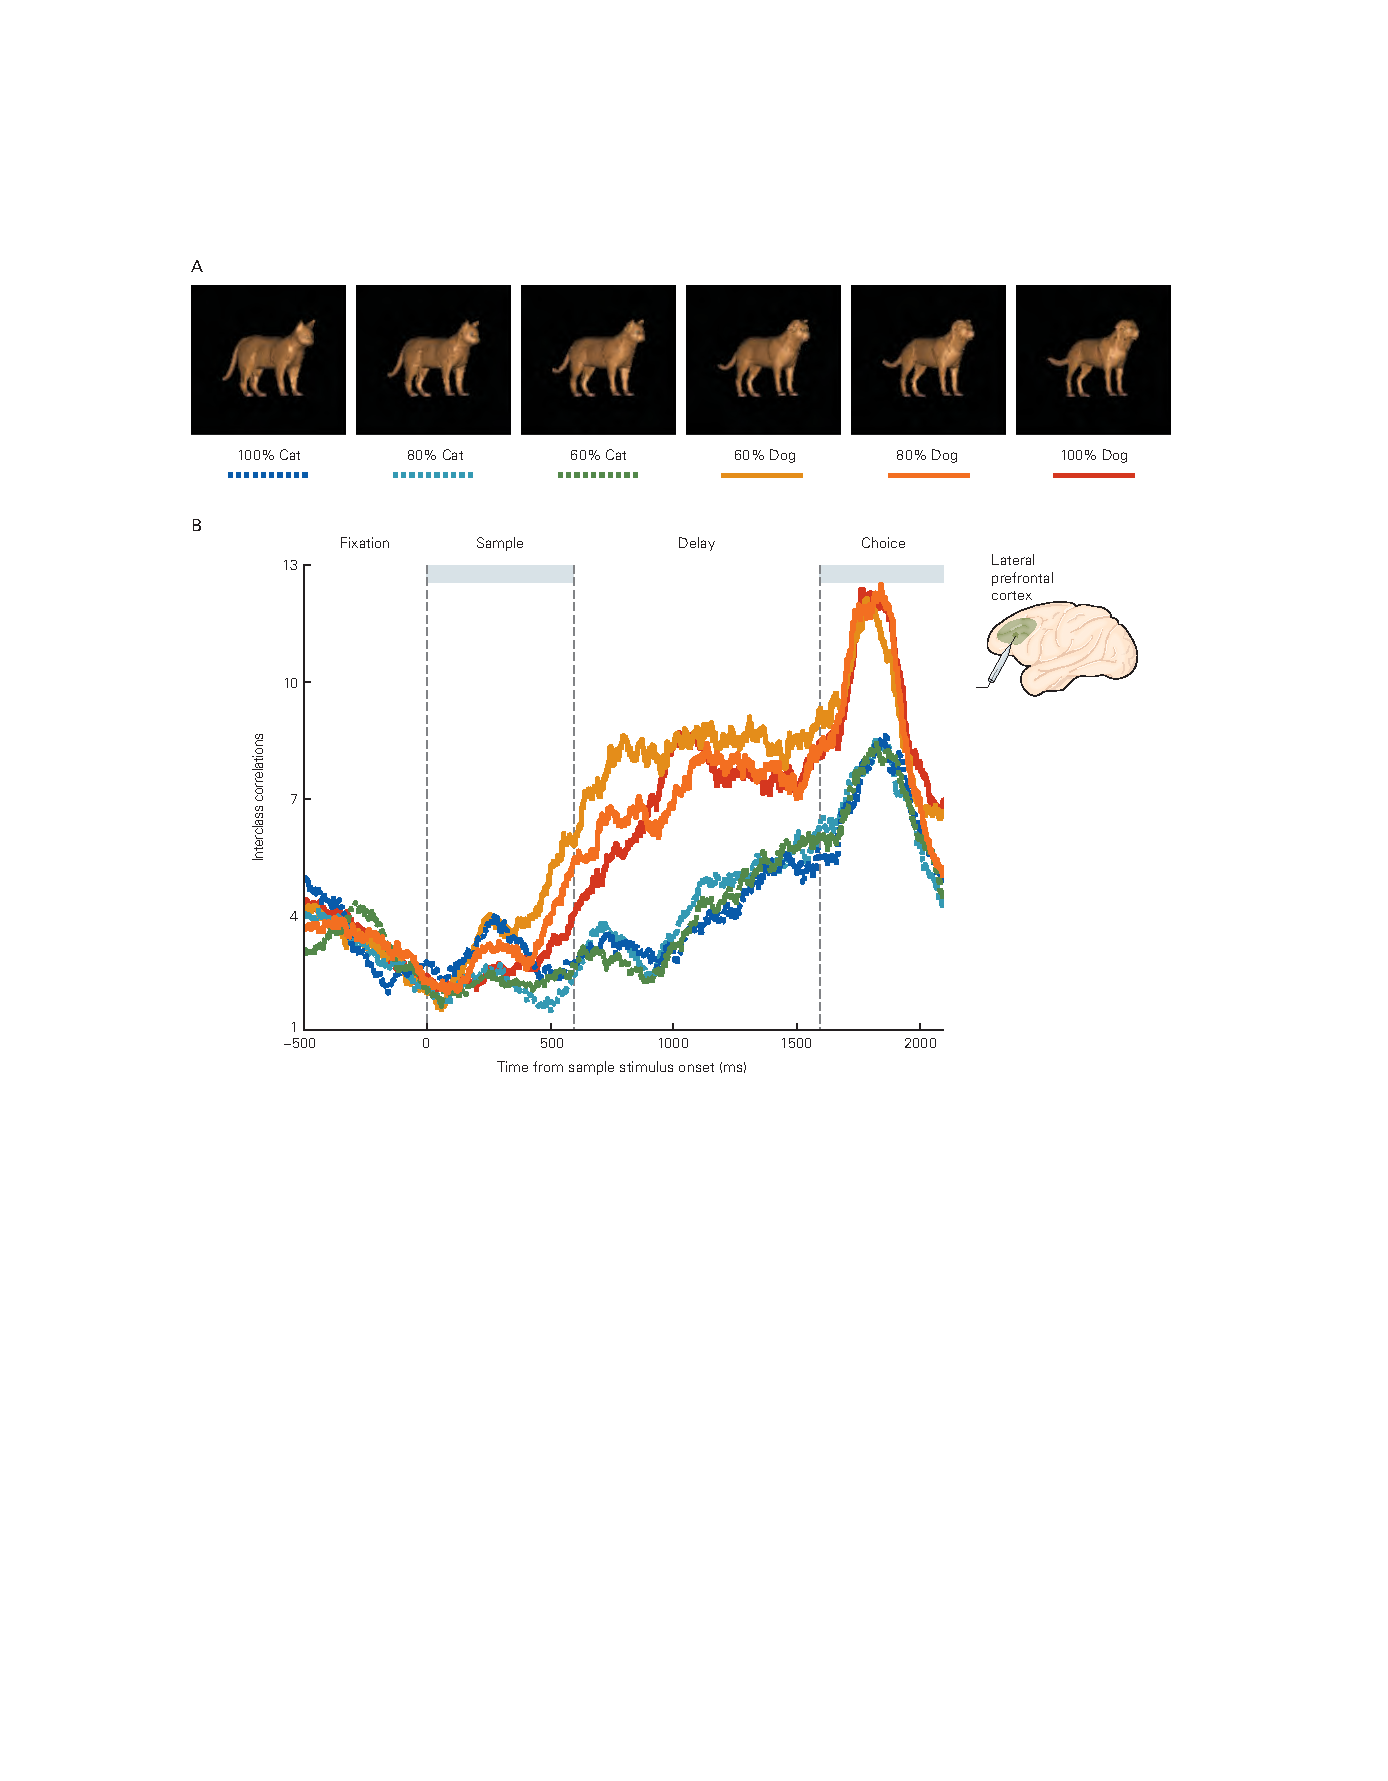
\includegraphics[width=0.9\linewidth]{chap24/fig_24_8}
	\caption{分类感知的神经编码。 (经许可转载自 Freedman 等人,2002 年。) A. 这些图像以不同的比例组合了猫和狗的特征。 如果图像具有猫或狗的 50\% 或更多特征,猴子会被训练将其归类为猫或狗。 B. 周围刺激时间直方图说明前额皮质神经元对 A 部分所示图像的反应。神经元对猫图像(100\%、80\% 和 60\%)的反应比对狗图像(60\%)的反应弱得多 、80\% 和 100\%)。 尽管视网膜图像的差异与类别之间的视网膜图像差异一样大,甚至更大,但对同一类别图像的反应非常相似。 因此,该单元格是特定于类别的。 这种特定于类别的反应在外侧前额叶皮层的视觉神经元中很常见。}
	\label{fig:24_8}
\end{figure}


类别特异性的不症有时会遵循颞叶的损害,这一事实表明,颞皮层中有神经元类别选择性,类别是类似于前额叶皮层中神经元的神经元。
颞皮层中的面部选择性细胞似乎符合此标准,因为它们对一系列面部的反应通常相似。
然而,这些可能构成一种特殊情况,而对于大多数刺激条件,类别选择性反应可能是前额叶皮层中神经元的特征,在额叶皮层中,视觉反应更常见于刺激的行为意义。



\section{视觉记忆是高级视觉处理的一个组成部分}

视觉体验可以作为记忆存储,视觉记忆会影响传入的视觉信息的处理。
对象识别特别依赖于观察者以前在对象上的经历。
因此,必须通过经验来修改对象识别的下颞皮层对物体识别的贡献。


关于经验在视觉感知中的作用的研究集中在两种不同类型的经验丰富的可塑性上。
一个源于反复的暴露或实践,这会改善视觉歧视和对象识别能力。
这些依赖经验的变化构成了一种被称为感知学习的隐性学习形式(第~\ref{chap:chap23}~章)。
另一个发生在与显式学习的存储,可以有意识地回忆的事实或事件的学习有关(第~\ref{chap:chap54}~章)。



\subsection{隐式视觉学习导致神经元反应选择性的变化}

通过经验来区分复杂的视觉刺激的能力是高度修改的。
例如,在汽车模型之间进行良好差异的个人提高了识别这种差异的能力。


在下颞皮层中,复杂对象的神经元选择性可以发生变化,与区分对象的能力相似之处。
例如,在Logothetis及其同事的一项研究中,对猴子进行了训练,可以从对象的二维视图中识别出新颖的三维物体,例如随机弯曲的线形式。
广泛的培训导致了从二维观点识别对象的能力的明显提高。
训练后,发现一群神经元对前面的观点表现出明显的选择性,但对同一对象的其他二维观点没有明显的选择性(图 ~\ref{fig:24_9})。


\begin{figure}[htbp]
	\centering
	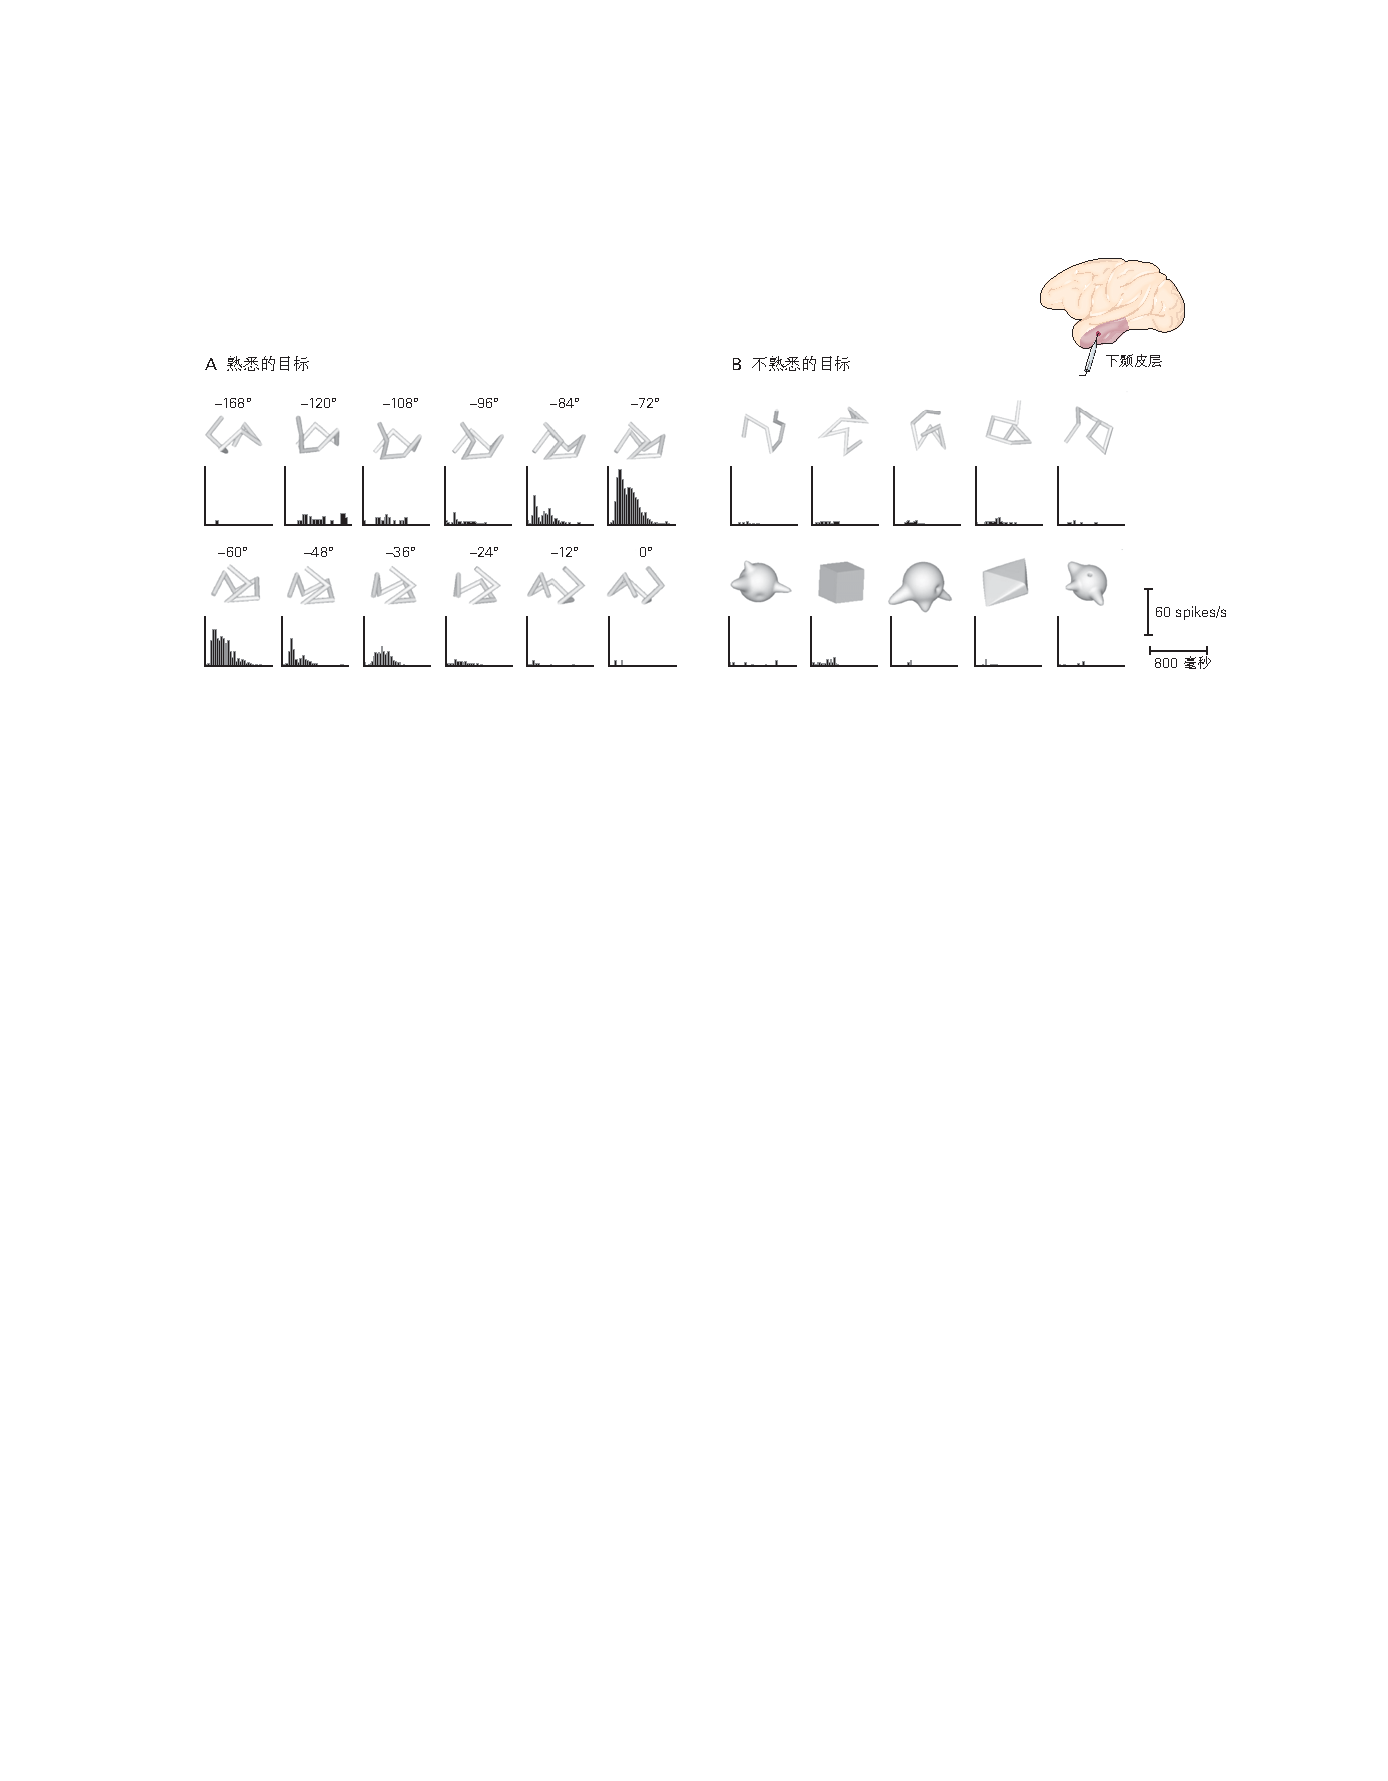
\includegraphics[width=0.9\linewidth]{chap24/fig_24_9}
	\caption{熟悉特定的复杂物体会导致下颞叶神经元对这些物体有选择性地做出反应。 (经许可转载自 Logothetis 和 Pauls 1995。版权所有 © 1995 Oxford University Press。) A. 训练猴子从电线的一组二维视图中识别随机弯曲的电线。 在连续的视图中,线形式旋转了 12°。 一旦识别性能在高水平上稳定下来,就会在呈现每个视图时从下颞叶皮层中的神经元进行记录。 周围刺激时间直方图显示典型神经元对每个视图的响应。 该神经元选择性地响应代表物体小范围旋转的视图。 B. 当用猴子不熟悉的两组刺激测试同一个神经元时,它对这些刺激中的任何一个都没有反应。}
	\label{fig:24_9}
\end{figure}


对猴子的其他研究表明,熟悉新面孔会改变下颞皮层中面部选择性神经元的调整。
同样,当动物具有由简单特征形成的新颖物体的经验时,下颞神经元就会对这些对象有选择性。
由于动物参与主动歧视或仅被动观察视觉刺激的原因,已经发现了这种神经元的变化,并且它们通常表现为神经选择性的锐化,而不是绝对发射速率的变化。
锐化恰恰是一种神经元变化,它可能是视觉刺激感知歧视的改善。



\subsection{视觉系统与工作记忆和长期记忆系统相互作用}

对象识别和学习是复杂的联系。
实际上,学习可以在下颞皮层中产生整个功能专业领域。 
例如,年轻学习以将特定形状(例如,数字符号)与特定奖励大小相关联的猴子会发展出处理这些特定形状的专业大脑区域。
这些大脑区域靠近前面讨论的颞叶面部斑块。


已经研究了有关视力与记忆之间相互作用的两个问题。
首先,如何在短期工作记忆中维护视觉信息?
工作记忆的容量有限,在计算机操作系统中像缓冲区一样起作用,并且长期记忆中的合并容易受到干扰(第 ~\ref{chap:chap54}~章)。
其次,如何存储和召回它们之间的长期视觉记忆及其之间的关联?


在视觉延迟响应任务中,需要访问超出刺激持续时间的刺激信息(方框24-1),在延迟期间,下颞皮层和前额叶皮层的许多与视觉相关的神经元在延迟期间都在继续触发。
这种延迟周期活动被认为可以将信息保持在短期工作记忆中(图~\ref{fig:24_11})。
下时间和前额叶皮层中的延迟周期活性在许多方面有所不同。
首先,下颞皮层中的活动与视觉模式和颜色信息的短期存储有关,而前额叶皮层的活动编码视觉空间信息以及从其他感觉方式中获得的信息。
下颞皮层中的延迟周期活性似乎也与视觉感知密切相关,因为它编码了样本图像,但是可以通过另一个图像的外观来消除。


\begin{figure}[htbp]
	\centering
	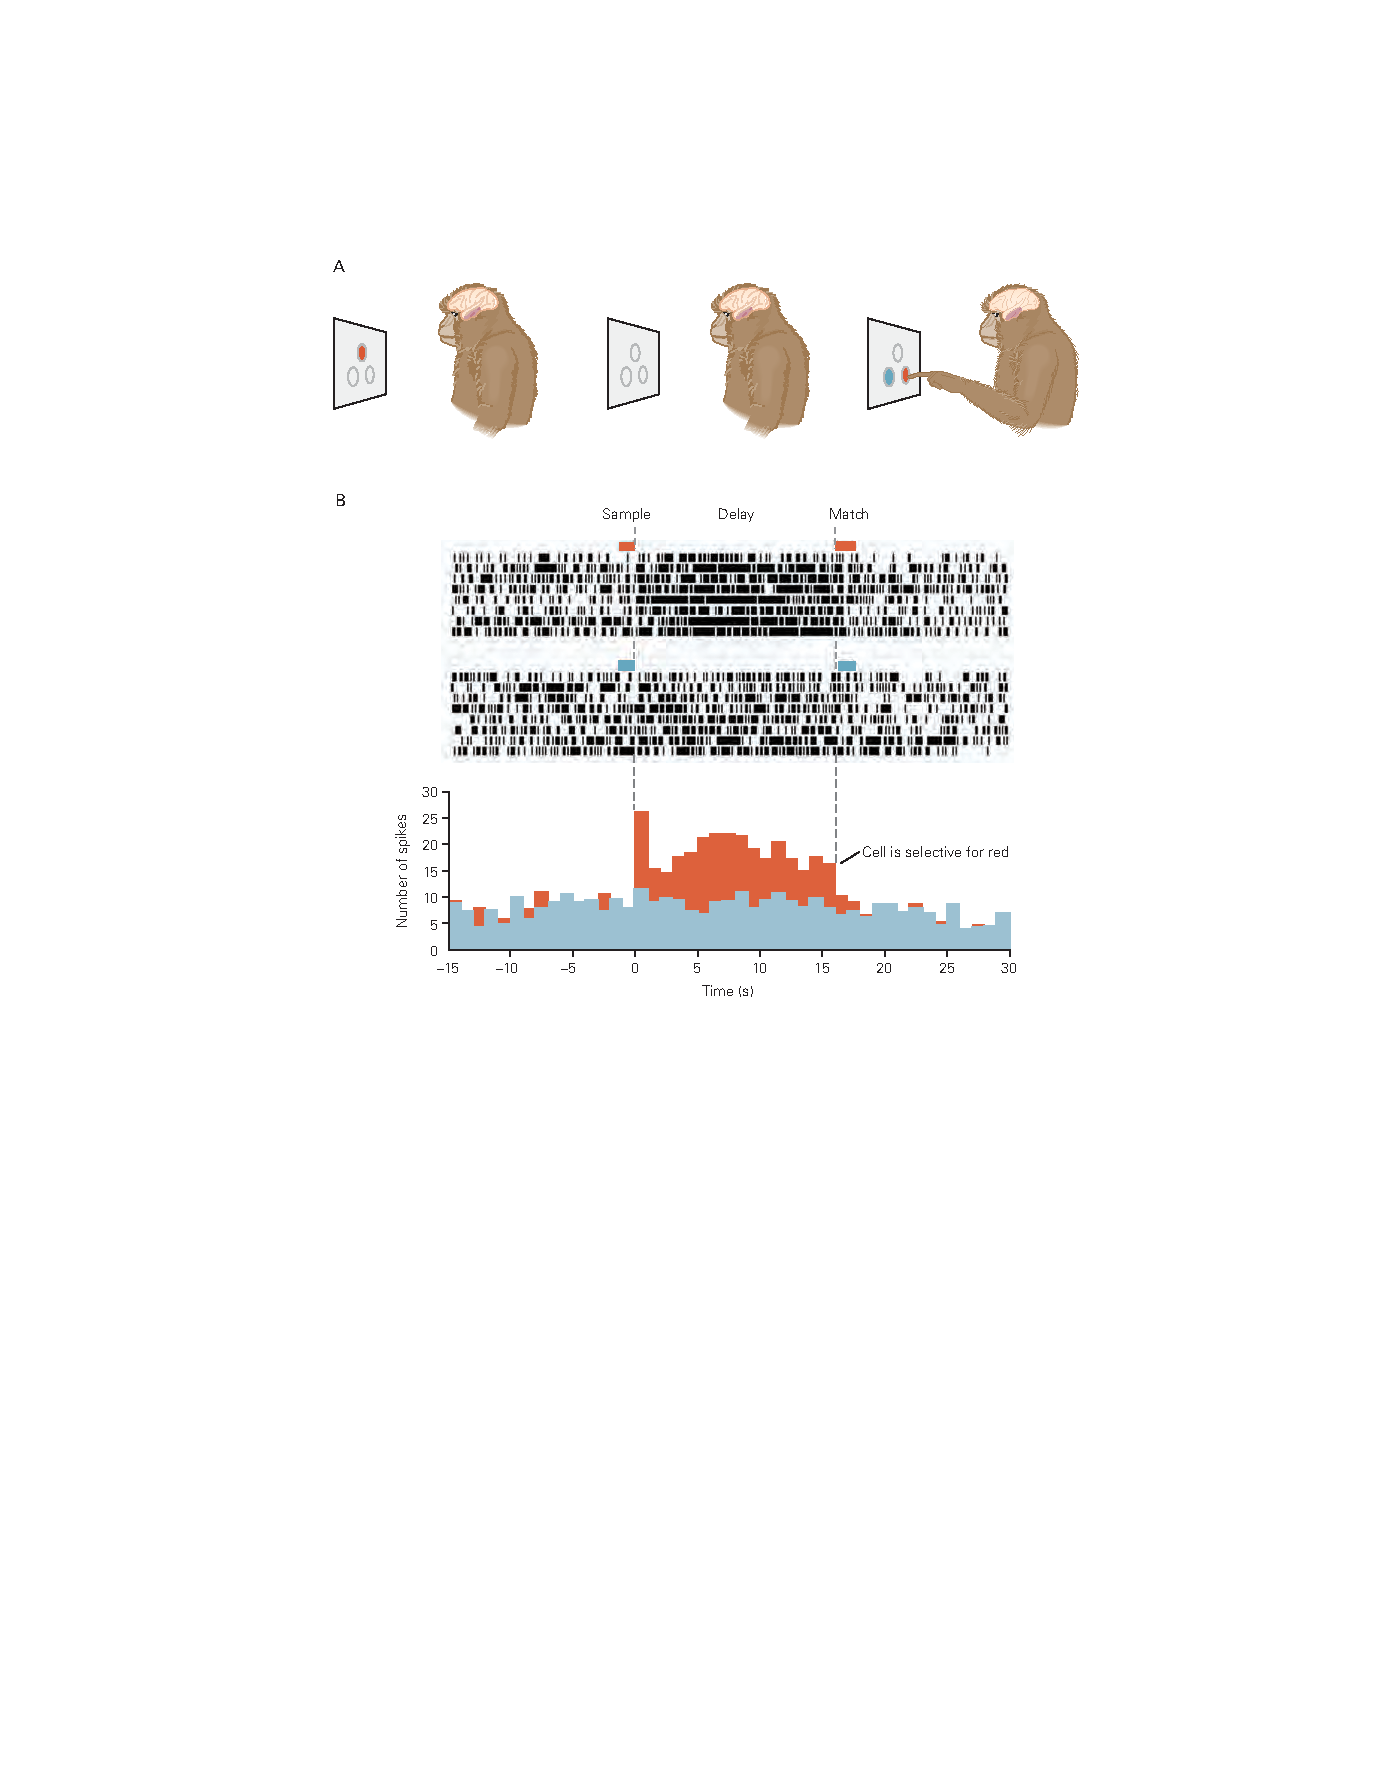
\includegraphics[width=0.75\linewidth]{chap24/fig_24_11}
	\caption{当对象保存在工作记忆中时,表示对象的神经活动就会持续。 (经许可转载自 Fuster 和 Jervey 1982。版权所有 © 1982 Society for Neuroscience。) A. 训练猴子执行颜色匹配样本任务。 例如,首先呈现红色刺激,然后动物必须从许多有色刺激中选择红色刺激。 该任务在样本显示和匹配之间加入了短暂的延迟(1-2 秒),在此期间,有关正确目标颜色的信息必须保留在工作记忆中。 猴子大脑中的紫色区域表示下颞叶皮层。 B. Peristimulus 时间直方图和动作电位光栅图说明了在延迟匹配样本任务期间下颞叶皮层中单个神经元的反应。 上面的记录来自样本为红色的试验,下面的记录来自样本为绿色的试验(此处显示为蓝色)。 录音显示细胞优先响应红色刺激。 在使用绿色样本的试验中,神经元的活动没有改变,而在使用红色样本的试验中,细胞在样本出现后表现出短暂的活动爆发,并在整个延迟期间持续放电。 下颞叶和前额皮层中的许多视觉神经元都表现出这种行为。}
	\label{fig:24_11}
\end{figure}


相比之下,在前额叶皮层中,延迟周期活动更多地取决于任务要求,并且不会因间歇性感觉输入而终止,这表明它可能在召回长期记忆中起作用。
Earl Miller及其同事的实验支持了这一观点。
在这些实验中,对猴子进行了培训以将多对物体相关联。 
然后,他们使用以下程序对他们是否学会了这些成对关联进行测试。
首先,提出了一个(示例)对象; 然后,短暂延迟后,出现了第二个(测试)对象。
指示猴子指示测试对象是否是上一次训练期间与样品配对的对象。


有两种可能解决此任务的方法。
在延迟期间,动物可以使用感官代码,并保留样本对象的在线表示,直到测试对象出现为止,或者可以记住样本对象的副词,并将有关关联对象的信息保留在“潜在代码”中 可能显示为测试对象的内容。
值得注意的是,在延迟期间,神经元活性似乎从一种过渡到另一个。
前额叶皮层中的神经元最初编码样本对象的感觉属性(刚刚看到的对象),但后来开始编码预期的(相关)对象。 
正如我们将看到的那样,前额叶皮层中的这种前瞻性编码可能是下颞皮层的自上而下信号的来源,激活代表预期对象的神经元,从而引起对该对象的有意识回忆。


在视觉刺激之间记忆的关联的背景下,已经广泛探索了长期声明性记忆存储与视觉处理之间的关系。
一个多世纪以前,美国实验心理学学院的创始人威廉·詹姆斯(William James)建议,学习视觉关联可能是通过编码个体刺激的神经元之间的连通性来介导的。 为了检验这一假设,托马斯·奥尔布赖特(Thomas Albright)及其同事训练猴子与没有事先物理或语义相关性的物体对相关。
后来对猴子进行了测试,同时进行了下颞皮层中神经元的细胞外记录。
已经配对的对象通常会引起类似的神经元反应,这是人们期望的,如果功能连接得到增强,而不成对象引起的响应是无关的。
猴子正在学习新的视觉关联时,来自单个下颞神经元的记录表明,在训练过程中,细胞对配对对象的反应变得更加相似(图~\ref{fig:24_12})。
最重要的是,神经元活动的变化发生在行为变化的时间表上,而神经活动的变化取决于成功学习。


\begin{figure}[htbp]
	\centering
	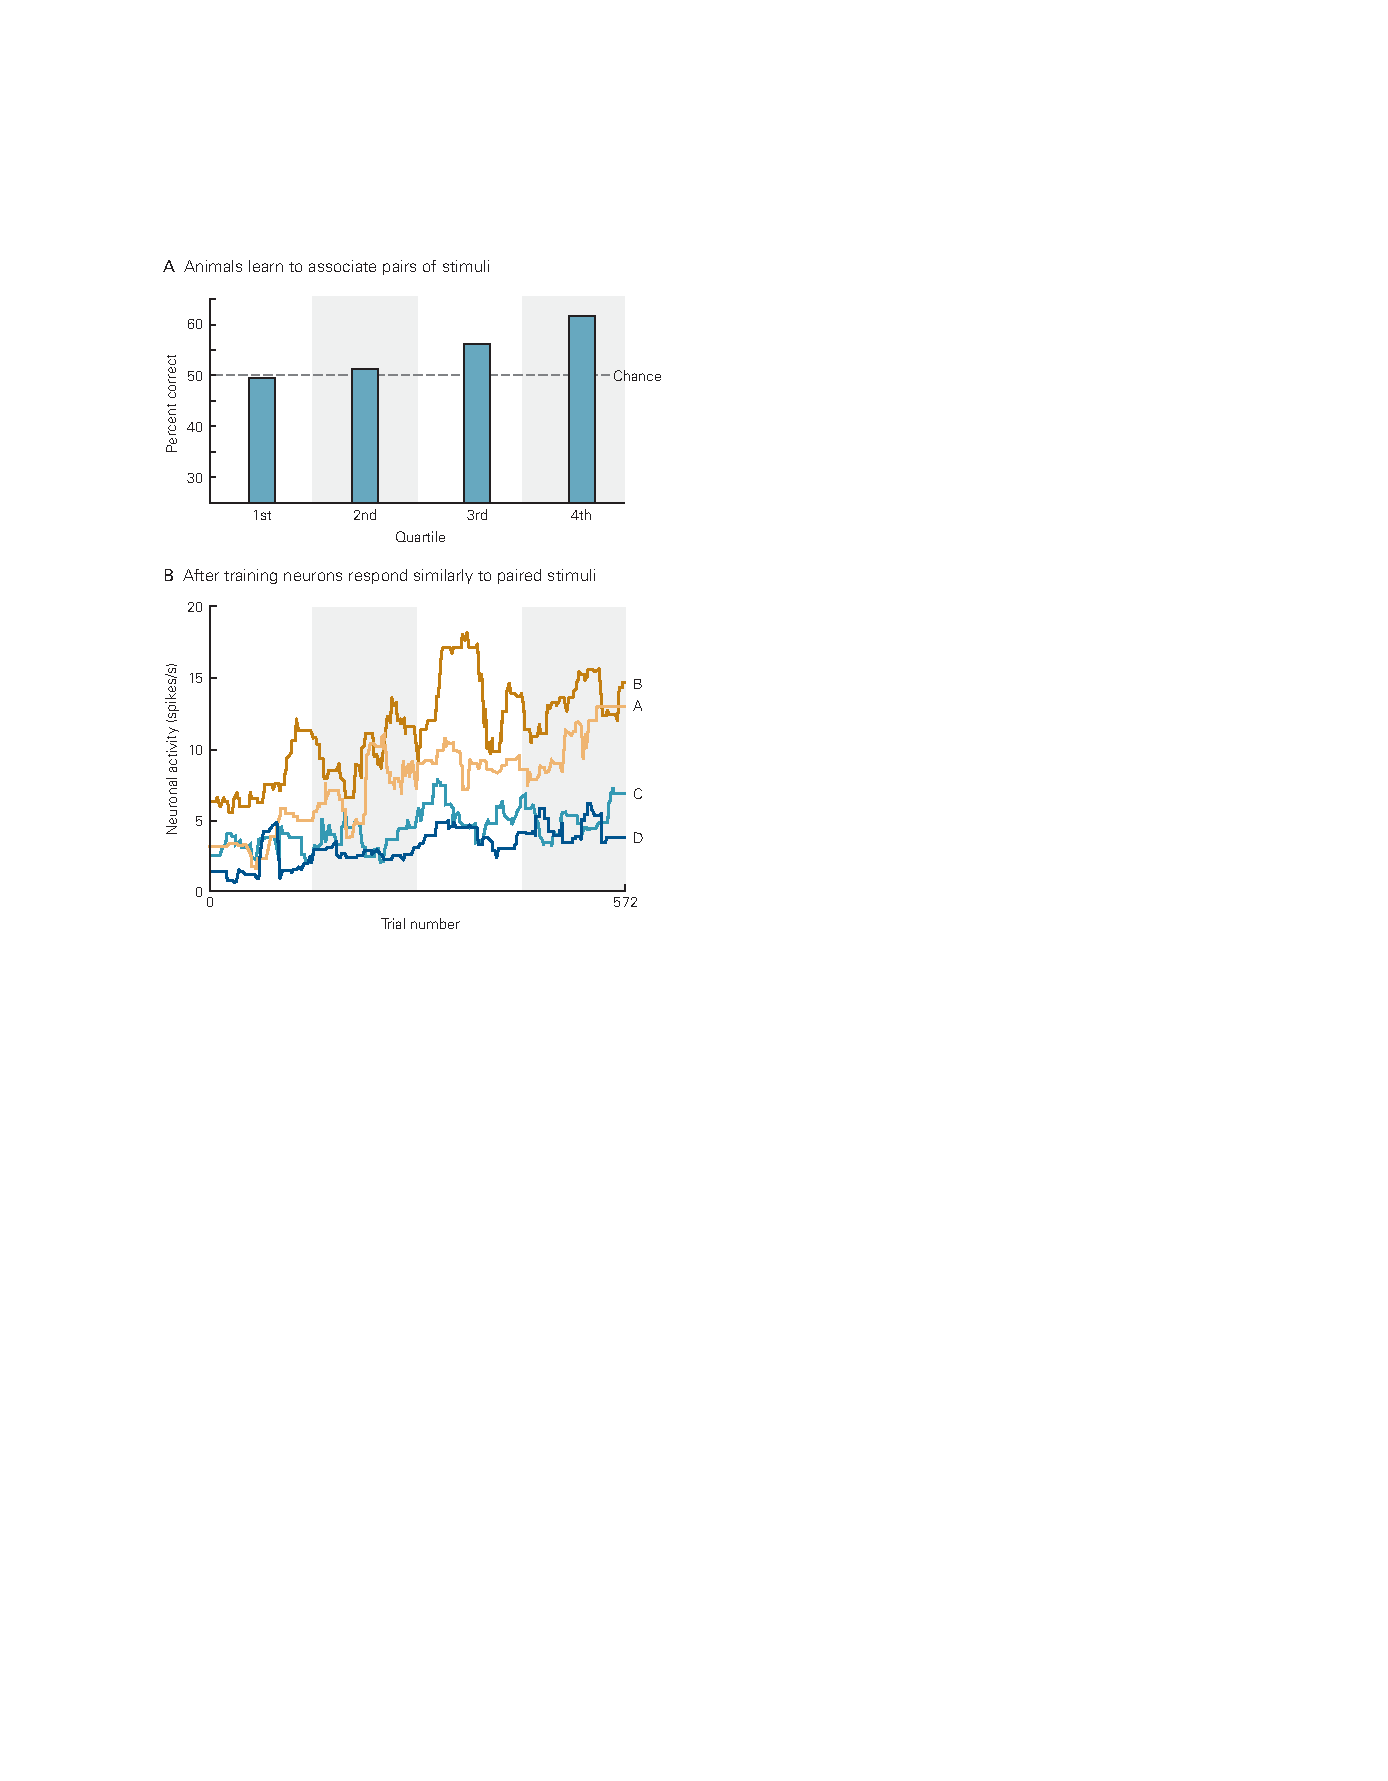
\includegraphics[width=0.5\linewidth]{chap24/fig_24_12}
	\caption{物体识别与联想记忆有关。猴子学会了视觉刺激对之间的关联,同时从下颞叶皮层的神经元记录活动。 (经许可转载自 Messinger et al. 2001。© 2001 美国国家科学院。) A. 为单个训练课程(572 次试验)的每个四分位数绘制配对关联任务的行为表现。 向动物展示了四种新刺激(A、B、C、D),并且需要学习两种配对关联(A–B、C–D)。 正如预期的那样,性能开始时是偶然的(50\% 正确),并随着动物学会这些关联而逐渐攀升。 B. 在 A 部分描述的行为任务期间记录的下颞神经元的平均放电率。每条轨迹代表四种刺激之一(A、B、C 或 D)呈现期间的放电率。 对所有刺激的反应在一开始都是相似的。 随着配对关联的学习,对配对刺激 A 和 B 的神经元反应开始聚集在与对配对刺激 C 和 D 的反应不同的水平上。神经元的活动因此对应于两对之间的学习关联。}
	\label{fig:24_12}
\end{figure}


这些依赖于学习的颞皮层神经元刺激选择性的变化是长期的,这表明该皮层区域是关联视觉记忆的神经回路的一部分。
实验结果还支持这样一种观点,即通过代表相关刺激的神经元之间的突触连接强度的变化来迅速实现学习的关联。


我们知道,内侧颞叶的海马和新皮层区域(周围,内嗅和帕拉希波克宫皮层)对于获得关联视觉记忆以及下颞皮层的功能可塑性都是必不可少的。
实际上,Yasushi Miyashita及其同事的工作表明,上述成对神经元在周围皮层中比前颞皮层更为普遍。
因此,尽管学习改变了两个区域中神经元的刺激选择性,但视觉相关对之间的关联从下颞皮层到周围的皮层增长(图24-2C)。
海马和内侧颞叶可以促进在存储关联视觉记忆所需的下颞皮层中局部神经元回路的重组。
重组本身可能是由相关视觉刺激的时间巧合引发的Hebbian塑性形式(第~\ref{chap:chap49}~章)。



\section{视觉记忆的联想回忆依赖于处理视觉刺激的皮层神经元的自上而下的激活}

高级视觉处理的最吸引人的特征之一是,在视野中检测图像和同一图像的回忆在主观上相似。
前者取决于视觉信息的自下而上流,这是我们传统上认为的视觉。
相比之下,后者是自上而下的信息流的产物。
这种区别在解剖学上是准确的,但掩盖了以下事实:
在正常条件下,信号伴随着降临的信号,以产生视觉体验。


对关联视觉记忆的研究为视觉回忆的基础机制提供了宝贵的见解。
如我们所见,视觉关联记忆通过独立代表相关刺激的神经元之间的功能连通性的变化来存储在视觉皮层中。
这一变化的实际结果是,仅在学习之前对刺激A反应的神经元在这些刺激已关联后将对A和B响应(图 ~\ref{fig:24_13})。
刺激B激活A反应性神经元可以看作是刺激A自上而下的回忆的神经元相关。


\begin{figure}[htbp]
	\centering
	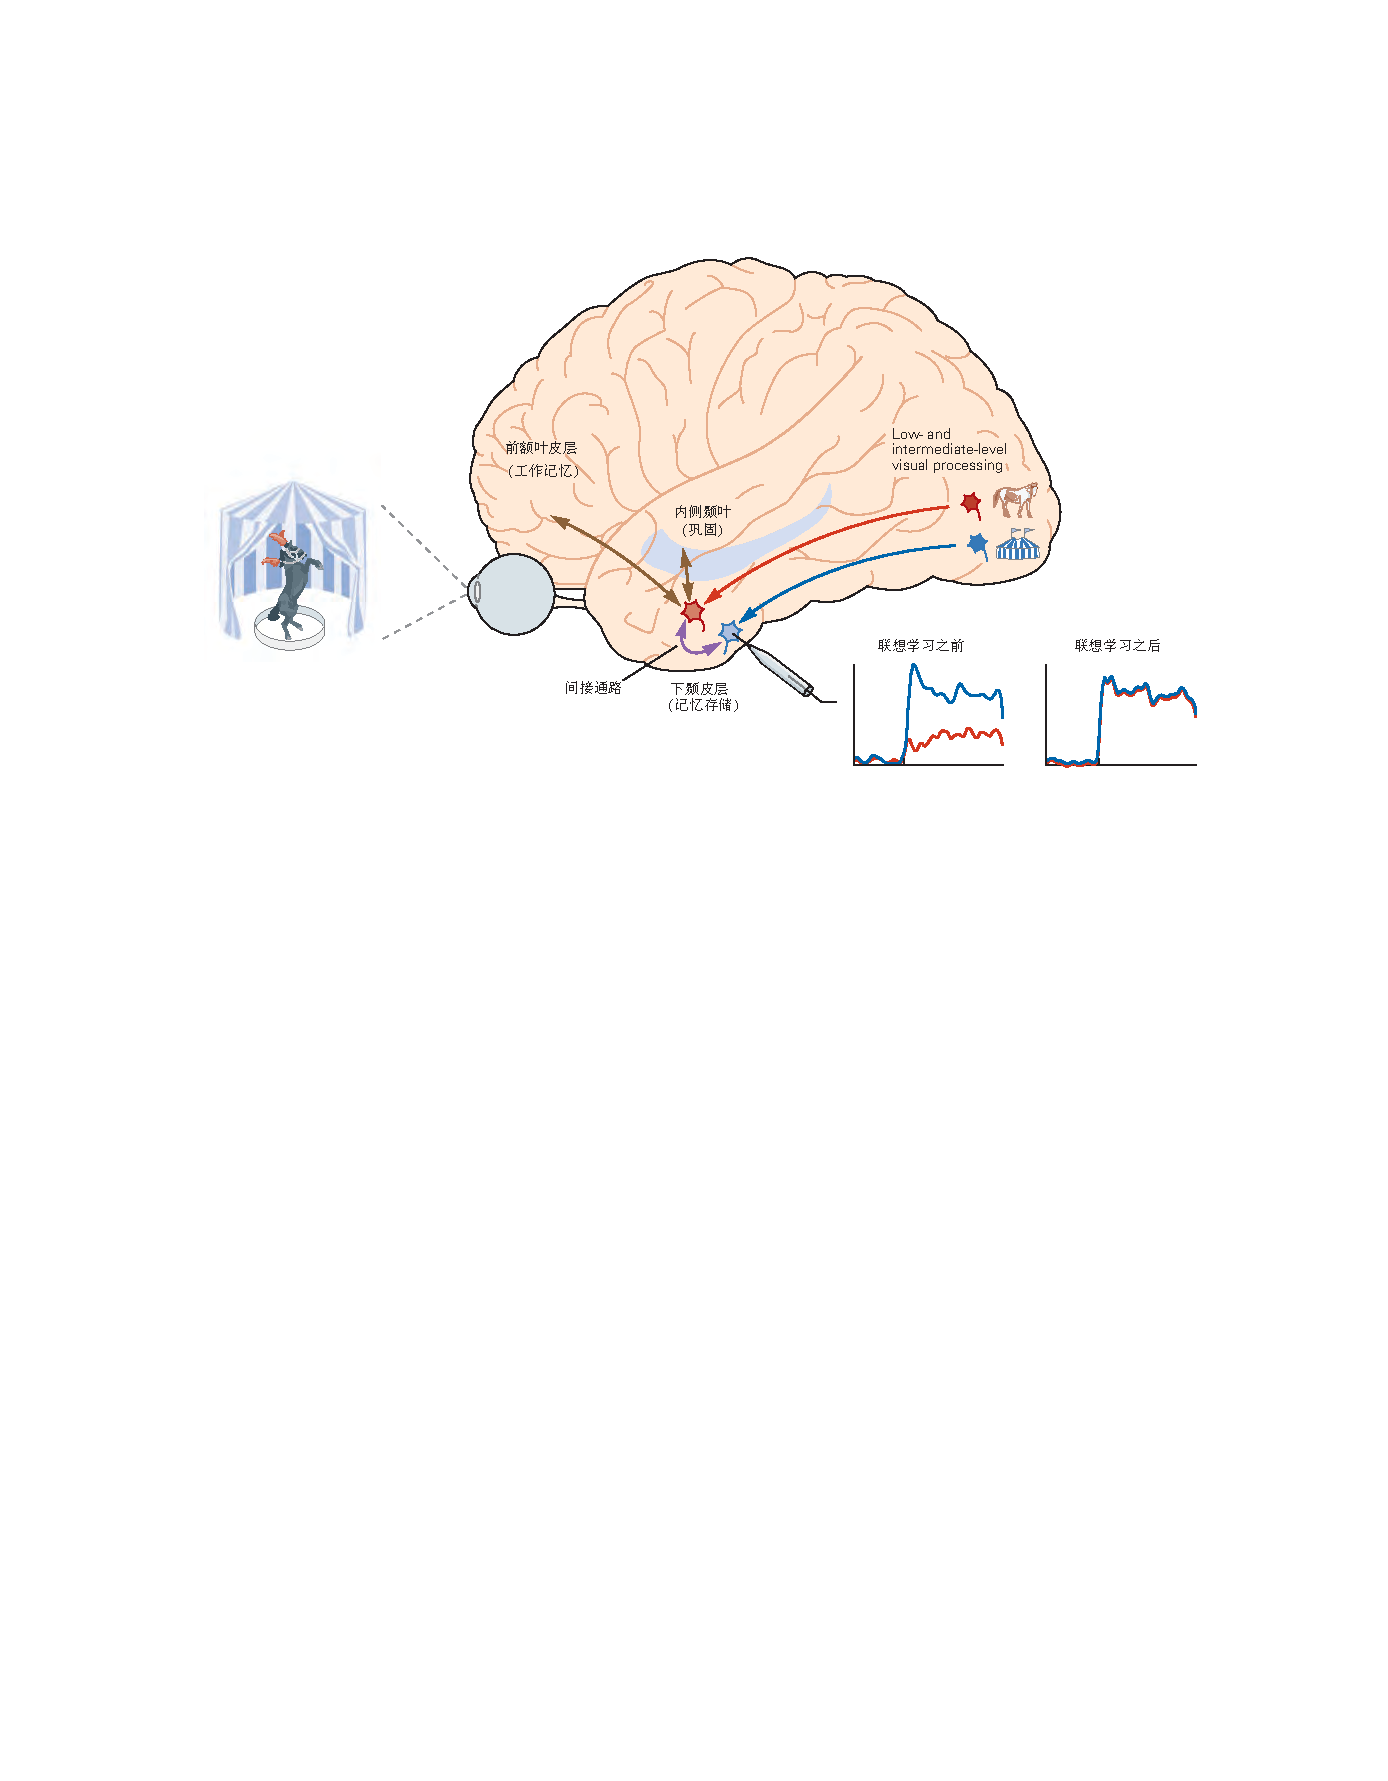
\includegraphics[width=0.9\linewidth]{chap24/fig_24_13}
	\caption{视觉联想和回忆的回路。自下而上的信号——传递观察者视野中物体信息的传入信号——被组合成下颞叶皮层的物体表征。在联想学习之前,一个神经元(蓝色)对马戏团的帐篷反应良好,但对马反应不佳。通过加强代表每个配对对象的神经元之间的连接(图中的间接通路),对象之间的习得关联在下颞叶皮层中被调节。因此,通过激活间接通路实现在马出现后回忆马戏团帐篷。 间接激活也可以由工作记忆的内容(来自前额叶皮层的反馈)触发。在正常情况下,视觉感知是对下颞叶神经元的直接和间接输入组合的产物。}
	\label{fig:24_13}
\end{figure}


下颞皮层中的神经元正好表现出这种行为。
与提示召回相关的活性与刺激的自下而上激活几乎相同。 
这些神经生理的发现得到了许多脑成像研究的支持,这些研究在提示和自发回忆期间发现了视觉皮层中的选择性活性。


尽管图像之间学到的关联可能通过下颞皮层的回路变化来存储,但这些回路的激活以进行有意识的回忆取决于前额叶皮层的输入。
下颞皮层可能会收到一对图像之一的传入信号,并传递到前额叶皮层,其中信息将在工作内存中维持。
如我们所见,在延迟匹配到样本任务的延迟期间,许多前额叶神经元的持续触发最初表示有关样本图像的信息,但会更改预期的相关图像。
从前额叶皮层到下颞皮层的信号将有选择地激活代表相关图像的神经元,并且该激活将构成视觉回忆的神经相关性。



\section{要点}

1.高级视觉的关键功能是对象识别。
对象识别具有含义的视觉感知。
正如著名的神经心理学家汉斯·卢卡斯·特伯(Hans-Lukas Teuber)曾经写过的那样,对象识别的失败“将以最纯粹的形式出现,作为一种正常的感知,以某种方式被剥夺了其含义。” 


2.对象识别很困难,这主要是由于外观变化,位置,距离,方向或照明条件的变化,可能会使外观相似的不同对象。
建立模仿灵长类动物对象识别能力的计算机模型是当前和未来研究的主要挑战。


3.对象识别依赖于称为下颞皮层的颞叶区域。
达到次颞皮层的视觉信息已经通过低和中级视力的机制处理。


4.颞颞皮层的病变会导致视觉不适,这是识别对象的能力的损失。
具有匹配或复制复杂对象的敏感性不可抗力,与关联性gnosia区分开来,这是识别对象的含义或功能的能力的损害。
从病变或灭活区域的模式中预测不可思议的确切性质,从而从理解相关性到神经对象表示的原因,是对象识别和神经病学领域的主要目标。 


5.下颞皮层中的单个细胞可以高度形状选择性,并有选择地对手或面部反应。他们可以在位置,大小甚至旋转之间保持选择性 - 可能解释感知恒定的专业。


6.上颞皮层包括迄今尚未数量的具有非常不同的功能专业的区域。
尽管整个组织的功能逻辑尚不清楚,但我们确实知道具有相似选择性组的细胞进入皮层柱,并且面部细胞被组织成称为面部区域的较大单元。 


7.面部识别受到多个面部区域的支持,每个面积都有独特的功能专业化。
面部区域有选择性地结合在一起,形成面部处理网络,该网络已成为高级视觉的模型系统。


8.上颞皮层与周围和偏头皮皮层相互连接,用于记忆形成,与杏仁核分配给对象的情感价,以及用于对象分类和视觉工作记忆的前额叶皮层。
如果将关联记忆存储为神经元之间的连接模式,那么海马和内侧颞叶的新皮层结构的特定贡献是什么,以及通过哪种细胞机制施加影响?
分子遗传学,细胞,神经生理和行为方法的汇合有望解决这些问题和其他问题。


9.对象被视为类别的成员。
这简化了适当的行为的选择,这通常不取决于刺激细节。 具有分类选择性的神经元在背侧前额叶皮层(下颞皮层的主要投影位点)中发现。


10.对象识别取决于过去的经验。
感知学习可以提高区分复杂物体和颞下皮层中的神经选择性的能力。


11.可以在短期工作记忆中保存视觉信息,以超过感觉刺激的持续时间。
刺激消失后,时间和额叶皮层中的神经元可以表现出延迟 - 周期活性。
这些网络如何建立保持信息在线的能力是一个悬而未决的问题。


12.高级视觉信息处理随自上而下的调制而变化。
图像的感官体验和记忆中相同的刺激的回忆在主观上相似。
下颞皮层中的神经元在自下而上激活和提示回忆中表现出相似的活性。


